\documentclass[fleqn,10pt]{wlscirep}
\usepackage[utf8]{inputenc}
\usepackage[T1]{fontenc}
\usepackage{placeins}
\usepackage{amsmath}
\usepackage{amssymb}
\usepackage[singlelinecheck=false,justification=justified,font=normalsize,labelfont=bf]{caption}
\usepackage{pdflscape}
\usepackage{graphicx}
\usepackage{lineno}
\usepackage{multirow}
\usepackage{csquotes}
\usepackage{xcolor}
\usepackage{hyperref}
\usepackage{algorithm}
\usepackage{algorithmic}
\usepackage{booktabs}

% natbib provides \citep and \citet natively (loaded by wlscirep.cls)

\title{Thinking With Models Through Simulation}

\author[1,*]{Kenny Yu}
\affil[1]{KU Leuven, Leuven, Belgium}
\affil[*]{kenny.yu@kuleuven.be}

\begin{abstract}
Computational models are central to behavioral science, yet a gap persists between knowing how to build a model and knowing how to \emph{think} with one. This tutorial in methodological reasoning introduces the Simulation Thinking Cycle, a six-step framework (Question, Formalize, Predict, Simulate, Surprise, Reflect) that structures simulation as a discipline of theoretical reasoning rather than a purely computational technique. Through worked examples using associative learning models, I develop six thinking skills: formulating simulatable questions, recognizing implicit commitments, discovering hidden predictions, designing critical experiments, evaluating robustness across parameter spaces, and bridging idealized predictions to realistic experiments. Three methodological contributions are emphasized: a commitment anatomy that decomposes models into core claims, auxiliary assumptions, and implementation choices (clarifying what a failed prediction actually tests); the demonstration that observation functions can qualitatively alter which model appears to fit data; and a distinction between structural and parametric predictions that separates theoretical claims from artifacts of parameterization. All skills are demonstrated through annotated R code with prediction checkpoints and hands-on exercises. Although the running examples use the Rescorla-Wagner and Mackintosh models, the techniques generalize to other computational models in behavioral science. All code and materials are available at \url{https://osf.io/f97rz/}.
\end{abstract}

\begin{document}
\flushbottom
\maketitle
\thispagestyle{empty}

\begin{linenumbers}

\section*{Introduction: Simulation as Theoretical Reasoning}

Simulation is a discipline of theoretical reasoning. When a researcher translates a verbal theory into executable code and runs it, something qualitatively different from verbal reasoning occurs: assumptions that were vague become explicit, predictions that were approximate become exact, and the gap between what the theory actually says and what the theorist thought it said becomes visible. This tutorial develops that discipline. Through worked examples and a structured six-step workflow, it treats simulation not as a preprocessing step before model fitting but as the core intellectual practice through which a theorist comes to understand what a theory actually claims.

A computational model is not a miniature replica of the world. It is an organized argument about what matters, what can be ignored, and what mechanisms are sufficient to produce the behavior of interest \citep{winsberg2010science}. To build a model is to make a series of commitments: which entities exist, how they interact, what changes over time, and what remains fixed. Every inclusion is a theoretical claim; every omission is equally loaded, an implicit argument that certain features of the real system do not matter for the question at hand. To simulate a model is to externalize counterfactual reasoning, to ask ``if the world were organized by these particular assumptions, what would follow?'' and to receive an answer that is a deductive consequence of those assumptions, not an empirical observation subject to noise or confounds. When a simulation surprises the researcher, the surprise reveals a gap between the theory's actual content and the researcher's interpretation of it. Because the assumptions that matter depend on the question being asked, simulation thinking always begins with a question, and the question determines which commitments become load-bearing.

This kind of discipline is overdue. Across behavioral science, researchers routinely derive predictions from computational models by reading equations and reasoning informally about their implications \citep{oberauer2019addressing, robinaugh2021invisible}. The reasoning feels rigorous but often breaks down in ways that are hard to catch, in the presence of nonlinear dynamics, feedback loops, and multi-variable interactions. Human working memory can track one or two variables simultaneously; computational models often contain a dozen, evolving across hundreds of trials. When researchers reason informally about such systems, they unknowingly solve a different, simpler problem than the one the model actually poses \citep{smaldino2017models, meehl1990summaries}.

\subsection*{The Missing Skill}

Excellent resources now exist for implementing models \citep{wilson2019ten, heathcote2015introduction}, fitting them to data \citep{farrell2018computational, lee2013bayesian}, and comparing them statistically \citep{wagenmakers2004aic, myung2003tutorial}. These resources answer an important question: how does one build and evaluate a model? But building a model and thinking with one are different activities, and the second has received far less attention.

Building a model requires both engineering skill and theoretical judgment. But there is a further intellectual practice, thinking \emph{with} a model, that goes beyond construction: it requires translating vague verbal intuitions into precise, executable commitments and then confronting the consequences of those commitments with genuine intellectual honesty \citep{guest2021computational, vanrooij2021theory, smaldino2020translate}. In that confrontation, one discovers assumptions one did not know one was making, predictions one did not know the theory entailed, and boundary conditions never previously considered. A model encodes a hypothesis about how a system works. Running that model forward in time reveals what the hypothesis actually entails \citep{lewandowsky1993role, mcclelland2009place}.

\citet{wilson2019ten} advise researchers to ``simulate, simulate, simulate'' as Rule~3 of their ten-step modeling guide. But the focus of those resources is the full pipeline from model specification through parameter estimation. The present tutorial treats simulation itself as the primary object: not a preprocessing step before fitting, but a structured reasoning practice with its own principles, its own characteristic pitfalls, and its own discipline of prediction and surprise.

\subsection*{The Simulation Thinking Cycle}

This paper develops that discipline through a structured workflow I call the Simulation Thinking Cycle (Figure~\ref{fig:cycle}). The cycle has six steps:
\begin{enumerate}
\item \emph{Question}: formulate a precise theoretical question that a simulation could answer.
\item \emph{Formalize}: translate the question into code (specifying model, design, parameters, and outcome variable), where every specification is a theoretical commitment.
\item \emph{Predict}: write down the expected result before running the simulation. This is the step most researchers skip and the one that makes simulation epistemically powerful: without a prediction, one never discovers that one's understanding of the theory is incomplete.
\item \emph{Simulate}: run the model.
\item \emph{Surprise}: compare the output to the prediction. Where they diverge, something has been learned about the gap between the theory's actual content and the researcher's interpretation of it.
\item \emph{Reflect}: ask which assumption produced the surprise, whether it is core or incidental, and what new question follows.
\end{enumerate}

The cycle reveals what a theory predicts; it does not reveal whether the theory is true. Its scope is the pre-empirical phase of modeling: the practice of using simulation to understand a theory's implications before confronting those implications with data. In practice, the cycle is embedded in a larger empirical arc: questions often originate from empirical puzzles, the Reflect step often generates hypotheses that demand experimental testing, and data from completed experiments feed new questions back into the cycle. But the cycle's core logic is pre-empirical; it concerns the relationship between the theorist and the theory, not yet between the theory and the world. The post-empirical phase (fitting, evaluating, revising) is treated by complementary tutorials \citep{wilson2019ten, farrell2018computational, lee2013bayesian}.

The cycle adapts the logic of strong inference \citep{platt1964strong} (formulate competing hypotheses, design a crucial experiment, carry it out, recycle) to the specific context of computational simulation, adding the Formalize and Predict steps that become necessary when models are too complex for verbal derivation. The paper walks through this cycle three times at progressively deeper levels: first with a single model, then with competing models, then across parameter spaces.
\subsection*{Learning Objectives}

After working through this tutorial, readers should be able to formalize vague theoretical questions into precise, simulatable ones; discover a theory's implicit commitments and hidden predictions through simulation; design critical experiments by simulating competing models to find divergence points; evaluate the robustness of conclusions across parameter and design spaces; and build virtual experiments that bridge idealized predictions to realistic data.

\subsection*{Prerequisites and Setup}

This tutorial assumes familiarity with basic R programming (loops, functions, vectors) and elementary statistics ($t$-tests, $p$-values). No prior knowledge of associative learning is needed; the models are introduced from scratch. The companion code requires R~$\geq$~4.0 with the \texttt{ggplot2} and \texttt{viridis} packages. All code is available at \url{https://osf.io/f97rz/}. Working through the full tutorial takes approximately 3--4 hours. The companion code is organized into modular scripts: \texttt{R/models.R} contains reusable model functions, \texttt{analysis/01\_blocking.R} through \texttt{analysis/05\_novel\_figures.R} contain section-by-section worked examples and figure generation, and \texttt{R/exercises.R} collects all hands-on exercises. Each analysis script can be run independently.

\begin{table}[t]
\centering
\small
\caption{Notation used throughout this tutorial.}
\label{tab:notation}
\begin{tabular}{cl}
\toprule
\textbf{Symbol} & \textbf{Meaning} \\
\midrule
$V_i$ & Associative strength of cue $i$ \\
$\alpha_i$ & Salience (RW) or attention (Mackintosh) for cue $i$ \\
$\beta$ & Outcome-tied learning rate (RW) \\
$\lambda$ & Maximum associative strength (asymptote) \\
$\Sigma V$ & Summed associative strength of all present cues \\
$S_i$ & Fixed salience parameter (Mackintosh) \\
$\beta_{\text{up}}$, $\beta_{\text{down}}$ & Attention change rates (Mackintosh) \\
$\delta$ & Prediction error ($\lambda - \Sigma V$ in RW) \\
$\gamma$, $\theta$, $\phi$ & Observation function parameters \\
\bottomrule
\end{tabular}
\end{table}

\subsection*{Roadmap}

The tutorial is organized around progressively deeper passes through the cycle. Section~2 takes the reader through the first complete cycle with a single model, using blocking and overexpectation as worked examples and introducing the role of observation functions. Section~3 runs the cycle a second time with competing models, developing the commitment anatomy of a model and the practice of designing critical experiments that distinguish theories. Section~4 takes the cycle to the level of parameter spaces, separating structural predictions from parametric coincidences. Section~5 bridges idealized predictions to realistic experimental designs through virtual experiments and simulation-based power analysis. An interlude between Sections~5 and~6 applies the full cycle to a drift-diffusion model, demonstrating that the framework transfers beyond associative learning. Section~6 distills seven portable principles and addresses common pitfalls.

Throughout, I use the Rescorla-Wagner \citep{rescorla1972theory} and Mackintosh \citep{mackintosh1975theory} models as the running example. Readers need no prior expertise in associative learning; the models are introduced from scratch as they are needed. Every technique developed here applies to any computational model with equations and parameters: drift-diffusion models, Bayesian learners, reinforcement learning agents, or any other formal framework the reader brings from their own domain \citep{platt1964strong, smaldino2023modeling}.

\begin{figure}[t]
\centering
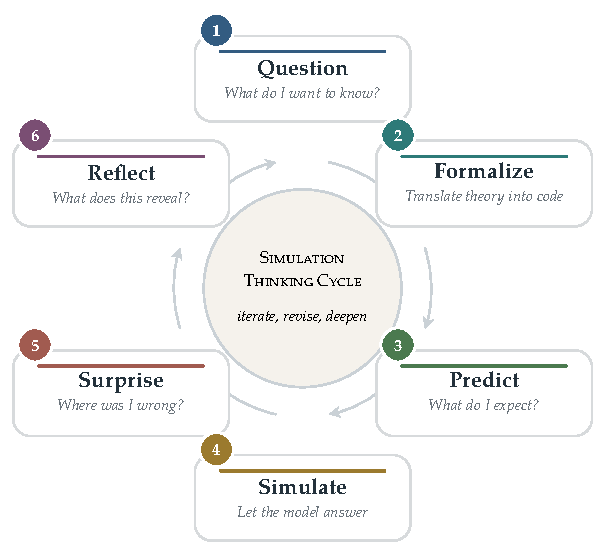
\includegraphics[width=0.55\linewidth]{Figures/fig1_cycle_diagram.pdf}
\caption{The Simulation Thinking Cycle. Each section of the paper walks through the cycle at a progressively deeper level: Section~2 uses a single model, Section~3 introduces competing models, Section~4 explores parameter spaces, and Section~5 bridges to experimental reality. The cycle is iterative: each round of reflection generates new questions, which may lead to further simulation cycles or to empirical testing.}
\label{fig:cycle}
\end{figure}

\setcounter{section}{1}
\section{From Words to Code: A First Dialogue with a Model}

The examples in this section and the next use deliberately simple, low-dimensional models: two cues, a handful of parameters, and deterministic dynamics. This transparency is pedagogical, not accidental. The logic of the Simulation Thinking Cycle is most visible when the model is simple enough that every assumption can be traced by hand and every prediction can be verified. Later model classes (neural networks, agent-based models, high-dimensional Bayesian models) may require approximate summaries, repeated simulations, or reduced diagnostics. The cycle scales, but its evidential force at each step depends on the model's transparency.

\subsection{The Formalization Ladder}

Theories exist at three levels of specificity, each requiring new commitments from the theorist \citep{smaldino2020translate}.

At the top sits the \emph{verbal theory}. Consider the statement: ``Learning is driven by prediction error.'' This sentence is intuitive, memorable, and profoundly ambiguous. What counts as a prediction? How is error computed? Across which stimuli? The sentence permits dozens of different formalizations, each making different predictions \citep{meehl1990summaries, vanrooij2021theory}.

One rung down, the verbal intuition crystallizes into a \emph{mathematical equation}. The Rescorla-Wagner update rule \citep{rescorla1972theory} provides a classic formalization:
\begin{equation}
\Delta V_i = \alpha_i \, \beta \, (\lambda - \Sigma V)
\label{eq:rw}
\end{equation}
where $V_i$ is the associative strength of cue $i$, $\alpha_i$ is its salience, $\beta$ is the learning rate tied to the outcome, $\lambda$ is the maximum associative strength, and $\Sigma V$ is the summed strength of all cues present on that trial. The equation constrains the theory substantially. Prediction error is now defined as $\lambda - \Sigma V$, a global error term shared across all present cues. But notice the choices made by omission: absent cues do not appear in $\Sigma V$ and are therefore not updated. And $\alpha_i$ is fixed; it does not change with experience. Both are theoretical commitments with consequences that will emerge shortly.

The final rung demands \emph{executable code}. To simulate Equation~\ref{eq:rw}, one must assign numerical values to $\alpha$, $\beta$, and $\lambda$, specify initial associative strengths, and define the trial sequence. The code permits no vagueness:
\begin{verbatim}
for (t in 1:n_trials) {
  cues_present <- design[[t]]$cues
  lambda       <- design[[t]]$lambda
  sum_V  <- sum(V[cues_present])
  delta  <- lambda - sum_V
  V[cues_present] <- V[cues_present] +
                     alpha[cues_present] * beta * delta
}
\end{verbatim}
Every line encodes a commitment. Only present cues are updated; absent cues are frozen. The error term is computed once and shared across all present cues. Salience $\alpha$ is read from a fixed vector and does not change. Five lines of code pin down more than a page of prose could. But note what is equally important: the choices the code does \emph{not} make. There is no fatigue process, no memory decay, no attentional fluctuation. Many omissions are as theoretically loaded as the explicit choices. Every abstraction is, at bottom, a claim about what can be safely set aside, whether because it is irrelevant to the question, intractable to compute, or likely to obscure the mechanism of interest: a claim that certain features of the real system do not matter for the question at hand.

For the single-cue case, Equation~\ref{eq:rw} admits a closed-form solution: $V_i(n) = \lambda[1-(1-\alpha_i\beta)^n]$, a negatively accelerated learning curve. With the parameters used here ($\alpha = 0.4$, $\beta = 0.3$), the effective learning rate is 0.12 per trial, giving $V_A \approx 0.72$ after 10 trials. But the moment a second cue enters the picture, the recursive dependencies between $V_A$ and $V_B$ make analytical solutions impractical. This is precisely where simulation becomes essential.

The epistemological power of simulation comes from this forced specificity. Every choice in the code is a theoretical commitment, and the commitments one makes without realizing it are often the ones that drive the most surprising predictions. When a simulation surprises the theorist, the productive response is to trace back up the ladder and ask which commitment, conscious or unconscious, produced the surprise.

\subsection{A First Thinking Cycle: Blocking}

The first complete pass through the Simulation Thinking Cycle uses a classic experimental design as its worked example. At each step, the phase of the cycle is marked explicitly.

\paragraph{Question.} If one signal already fully predicts an outcome, what can a newly added signal learn? In the language of Equation~\ref{eq:rw}: if cue A has been trained to high associative strength, and compound trials are then introduced where A and a novel cue B both precede the outcome, what happens to $V_B$? This question applies to any prediction-error model, not only associative learning \citep{sutton2018reinforcement, courville2006bayesian}.

\paragraph{Formalize.} Phase~1: 10 trials of A+ (cue A followed by the outcome). Phase~2: 10 trials of AB+ (compound of A and B followed by the outcome). Parameters: $\alpha_A = \alpha_B = 0.4$, $\beta = 0.3$, $\lambda = 1.0$, initial $V_A = V_B = 0$. Each choice is a commitment. These choices will be revisited in Section~4.
\begin{verbatim}
design <- c(
  make_trials("A", lambda=1, n=10, "Phase 1"),
  make_trials(c("A","B"), lambda=1, n=10, "Phase 2"))
results <- rw_simulate(design,
             alpha=c(A=0.4, B=0.4), beta=0.3)
\end{verbatim}

\paragraph{Predict.} Before examining the simulation output, the reader should pause for what I call a \emph{prediction checkpoint}: a deliberate moment of intellectual honesty that is central to simulation-based thinking. After Phase~2, will $V_B$ be approximately 0.5, approximately 0.3, or approximately 0.0? The reader should commit to an answer before reading on. The value of this exercise comes entirely from the possibility of being wrong.

\paragraph{Simulate.} Figure~\ref{fig:blocking} shows the results. During Phase~1, $V_A$ rises toward $\lambda$, reaching approximately 0.72 after 10 trials. In Phase~2, $V_B$ barely increases: after 10 compound trials, $V_B \approx 0.13$. Cue B, despite consistent pairing with the outcome, has learned very little.

To see why, consider a step-by-step trace of the computation. Table~\ref{tab:handtrace} shows the first three Phase~1 trials and the first two Phase~2 trials. During Phase~1, only A is present, and $V_A$ grows with negatively accelerated dynamics. The critical moment occurs at trial 11, the first compound trial. At this point $V_A = 0.722$ and $V_B = 0$, so the prediction error is $\delta = 1.0 - 0.722 = 0.278$. Both A and B receive the same small update of 0.033. By trial 12, $V_A$ has risen to 0.755, and the error has shrunk to $\delta = 0.212$. The updates are even smaller: $\Delta V_A = \Delta V_B = 0.025$. This pattern continues: each trial's error is smaller than the last, because A is absorbing the teaching signal before B can accumulate meaningful associative strength.

\begin{table}[t]
\centering
\small
\caption{Trial-by-trial hand trace of the Rescorla-Wagner model through the blocking design. Phase~1 trains A alone; Phase~2 introduces the compound AB. The key observation is that by the start of Phase~2, $V_A$ is already high enough that $\delta$ is small, leaving little learning signal for B.}
\label{tab:handtrace}
\begin{tabular}{ccccccc}
\toprule
Trial & Phase & Cues & $\Sigma V$ & $\delta$ & $\Delta V_A$ & $\Delta V_B$ \\
\midrule
1 & 1 & \{A\} & 0.000 & 1.000 & 0.120 & -- \\
2 & 1 & \{A\} & 0.120 & 0.880 & 0.106 & -- \\
3 & 1 & \{A\} & 0.226 & 0.774 & 0.093 & -- \\
\multicolumn{7}{c}{\emph{$\cdots$ (trials 4--10 omitted; $V_A$ reaches 0.722)}} \\
11 & 2 & \{A,B\} & 0.722 & 0.278 & 0.033 & 0.033 \\
12 & 2 & \{A,B\} & 0.789 & 0.211 & 0.025 & 0.025 \\
\bottomrule
\end{tabular}
\end{table}

As $V_A$ rises further toward $\lambda$, $\delta$ shrinks: a self-correcting cycle in which A's prior learning eliminates the teaching signal before B can benefit. The model does not distinguish which cue deserves credit; it only registers that the total prediction is accurate.

This is blocking \citep{kamin1969predictability}, and the Rescorla-Wagner model's ability to capture it was a landmark achievement \citep{rescorla1972theory}. The prediction error mechanism has neural correlates in dopamine signaling \citep{schultz1997neural}.

\paragraph{Surprise.} If the reader predicted $V_B \approx 0$, the intuition aligned with the model. If a higher value was predicted (and many researchers do, even those who can recite the RW equation), the discrepancy is epistemically valuable. The verbal understanding of ``prediction error drives learning'' did not prepare the reader for this specific quantitative consequence.

\emph{Exercise 1.} Change $\alpha$ to \texttt{c(A=0.9, B=0.9)} and rerun the blocking simulation. Does blocking become stronger or weaker? (Expected: stronger, because A learns faster in Phase~1, leaving even less error for B.) Then try \texttt{beta=1.0}: what happens?

\paragraph{Reflect.} Simulation externalizes counterfactual reasoning that is too complex for working memory to handle. The researcher is asking ``what would happen if the world were governed by these specific assumptions?'' but the question involves too many interacting variables for the answer to be derived mentally. Working memory cannot simultaneously track the evolving values of $V_A$ and $V_B$, the trial-by-trial prediction error, and its differential allocation across 20 sequential trials. The model can. This limitation is not specific to associative learning: any model involving multi-variable interactions over time generates dynamics that verbal reasoning cannot faithfully track.

When prediction and simulation disagree, the disagreement is between the researcher's understanding and the model's actual implications. Before simulation, the understanding of ``prediction error drives learning'' was a verbal paraphrase, a summary that captured the spirit but discarded the specifics. After simulation, the researcher has encountered one precise formalization of the theory, in its full, uncompromising specificity.

A simulation result is a \emph{deductive} consequence of the model's assumptions as specified and implemented. It is not empirical data, which is always uncertain, and it is not verbal reasoning, which is always approximate. Within a given formalization and implementation, the output follows necessarily from the premises \citep{winsberg2010science}. When a simulation surprises the researcher, the surprise is grounded in the implications of the implemented model, not in noise or informal approximation. An unexpected datum might reflect confounds or measurement error; an unexpected simulation result reflects the logical content of one specific formalization. This guarantee is conditional on correct implementation, and the model is only one possible formalization of the underlying verbal theory (see Section~3.3). But within those bounds, the surprise is warranted: the formalized model speaks more precisely than the theorist's unaided intuition.

A reasonable objection is that simulation is merely faster hand calculation. For the simplest case, this is true. But it becomes intractable for designs with multiple cues, multiple phases, or cue-specific dynamics. The three-phase critical test of Section~3 and the parameter sweeps of Section~4 are beyond analytical reach entirely. The ideal practice combines both: simulation discovers what the model predicts; analytical reasoning explains why \citep{navarro2021mathematical}.

\begin{figure}[t]
\centering
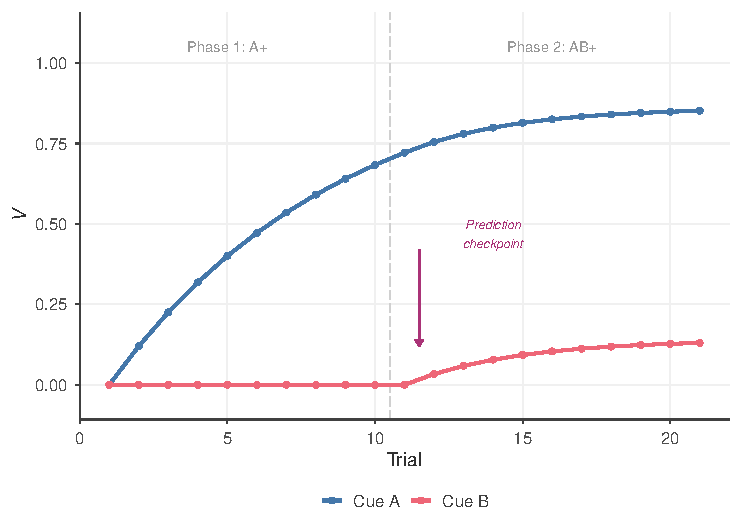
\includegraphics[width=0.7\linewidth]{Figures/fig2_blocking.pdf}
\caption{Blocking simulation using the Rescorla-Wagner model. During Phase~1 (A+), $V_A$ rises toward asymptote. During Phase~2 (AB+), $V_B$ remains near zero despite consistent pairing with the outcome. The arrow marks the prediction checkpoint.}
\label{fig:blocking}
\end{figure}

\subsection{From Internal State to Observable Behavior}

By the end of Phase~2, $V_A$ has risen to approximately 0.85, while $V_B$ remains near 0.13. Before continuing, I address a commitment that researchers often leave implicit. Throughout this section, $V$ has been treated as though it were directly observable. It is not. $V$ is an internal theoretical variable. To connect it to measurable behavior (response latency, response rate, choice probability), an \emph{observation function} is needed: a mapping from the model's internal state to the dependent variable actually recorded in an experiment.

This mapping is itself a theoretical commitment, and different choices can alter qualitative predictions. Common observation functions include a sigmoid (logistic) response function $P(\text{CR}) = 1/(1 + e^{-\gamma(V - \theta)})$, a threshold rule $P(\text{CR}) = \mathbf{1}[V > \theta]$, and a Luce choice rule $P(i) = e^{\phi V_i}/\sum_j e^{\phi V_j}$, where $\theta$ is a threshold, $\gamma$ controls sigmoid steepness, and $\phi$ is a sensitivity parameter.

To see why this matters concretely, consider the blocking results with $V_A = 0.85$ and $V_B = 0.13$ at the end of Phase~2. Under a sigmoid mapping ($\gamma=5$, $\theta=0.5$): $P(\text{CR}|A) = 0.85$ and $P(\text{CR}|B) = 0.14$, a clear behavioral difference. But with a lower threshold ($\theta=0.1$): $P(\text{CR}|B) = 0.54$; suddenly B produces a non-negligible response. Same model, same internal dynamics, but a different behavioral prediction because the observation function changed. Internal model variables must therefore be mapped to observables through an explicitly specified observation function. Whenever a model is simulated, one should specify this mapping and consider whether the conclusions survive alternative mappings.

To make this concrete, Table~\ref{tab:obsfun} shows how the same internal associative strengths from the blocking simulation map onto different behavioral predictions under three observation functions. The raw $V$ values suggest a graded difference between A and B. The sigmoid with a moderate threshold amplifies this into a near-categorical distinction. The strict threshold produces an all-or-nothing pattern. And the Luce choice rule, which normalizes across options, shows that B's relative probability of being chosen is far lower than the raw $V$ might suggest.

\begin{table}[t]
\centering
\small
\caption{Effect of observation function on behavioral predictions. The same internal associative strengths ($V_A = 0.85$, $V_B = 0.13$) produce qualitatively different behavioral patterns depending on the mapping from internal state to observable.}
\label{tab:obsfun}
\begin{tabular}{lcc}
\toprule
\textbf{Observation function} & $P(\text{response}|A)$ & $P(\text{response}|B)$ \\
\midrule
Raw $V$ (identity) & 0.85 & 0.13 \\
Sigmoid ($\gamma=5$, $\theta=0.5$) & 0.85 & 0.14 \\
Sigmoid ($\gamma=2$, $\theta=0.3$) & 0.75 & 0.42 \\
Threshold ($\theta=0.5$) & 1.00 & 0.00 \\
Threshold ($\theta=0.1$) & 1.00 & 1.00 \\
Luce choice ($\phi=3$) & 0.90 & 0.10 \\
\bottomrule
\end{tabular}
\end{table}

The observation function is not a minor technical detail. It represents a substantive theoretical claim about the relationship between internal learning and external behavior. In some experimental paradigms, the choice of observation function does not matter because the qualitative prediction is the same regardless. But in others (particularly those near the boundary between responding and not responding, as in the case of cue B after blocking), the observation function determines whether the model predicts a behavioral effect or not. Whenever simulation results are interpreted, the observation function should be stated explicitly, its consequences explored, and the robustness of conclusions across plausible alternative mappings assessed.

\emph{Exercise 2.} Apply a threshold observation function with $\theta = 0.5$ to the blocking results. Does B ever produce a conditioned response? Now try $\theta = 0.1$. (Use \texttt{obs\_sigmoid()} and \texttt{obs\_threshold()} from \texttt{R/models.R}.)

\subsection{Discovering Unanticipated Predictions}

The blocking example demonstrated one thinking skill: using simulation to check whether intuitive understanding of a model matches its actual predictions. A second, and in some ways more powerful, skill is using simulation to discover predictions that were never anticipated. Every model contains more predictions than its creator realized. Simulation is the tool for finding them.

Consider the following design. In Phase~1, cues A and B are each trained separately: A+ and B+ on alternating trials, 10 trials each. By Phase~1's end, $V_A \approx V_B \approx 0.72$. In Phase~2, compound trials: AB+. The outcome is still present. Both cues are still reinforced.

\emph{Prediction checkpoint.} Most people reason as follows: A and B are both reasonably well-learned; compounding them with the same outcome should not change much; $V_A$ and $V_B$ should remain stable or perhaps continue rising. The reader should commit to a prediction before continuing.

The simulation (Figure~\ref{fig:overexpectation}) reveals that both $V_A$ and $V_B$ \emph{decline} during Phase~2. They do not stabilize; they drop. The mechanism is the same prediction error rule operating in the opposite direction: $\delta = \lambda - (V_A + V_B) \approx 1.0 - 1.44 = -0.44$. The summed prediction exceeds the outcome. The negative error drives both associative strengths downward. Both cues lose strength despite continued reinforcement. This is overexpectation \citep{rescorla1970reduction, lattal1998overexpectation}. This prediction was not designed into the model; it fell out of the same mechanism that produced blocking, waiting to be discovered.

To trace the mechanism more precisely, consider the first compound trial. The design gives 10 trials per cue (alternating A+ and B+), so $V_A = 0.72$ and $V_B = 0.72$ at the end of Phase~1. Then $\Sigma V = 1.44$ and $\delta = 1.0 - 1.44 = -0.44$. The updates are $\Delta V_A = 0.4 \times 0.3 \times (-0.44) = -0.053$ and $\Delta V_B = -0.053$. Both cues lose associative strength on a single trial. On the next trial, $\Sigma V$ is smaller, so $\delta$ is less negative, and the decline decelerates. The system converges toward an equilibrium where $V_A + V_B = \lambda$, which means each cue settles at approximately $\lambda/2 = 0.5$ if both have equal salience.

This result is deeply counterintuitive. A cue that is consistently paired with an outcome \emph{loses} associative strength, not because reinforcement is withdrawn, but because the presence of another well-learned cue causes the summed prediction to overshoot. The practical implication is that combining two effective predictors can make each one less effective, a prediction that has been confirmed empirically \citep{rescorla1970reduction, lattal1998overexpectation}. Without simulation, this prediction is easy to overlook: the verbal statement ``prediction error drives learning'' does not advertise that two well-learned cues will lose associative strength when compounded.

The prediction space of a model is vastly larger than the predictions a theorist has explicitly considered. Researchers should take their own models, simulate designs they have never tested, and examine what emerges.

The predictions discovered through simulation have enhanced evidential value precisely because they are \emph{novel}, not used in constructing the model. In the philosophy of science, novel predictions can constitute more severe tests of a theory than retrodictions of known phenomena, because a theory that successfully predicts something it was not designed to explain has passed a test it could easily have failed \citep{mayo1996error}. Overexpectation was not built into the Rescorla-Wagner model; it fell out of a mechanism designed to explain other phenomena. When such a prediction is subsequently confirmed empirically, it provides stronger evidence for the model than a successful fit to the data that motivated the model's construction in the first place. Simulation is the tool that makes these novel predictions discoverable. The most valuable simulation results are those that are \emph{surprising but intelligible in retrospect}: unexpected when first encountered, yet fully traceable to the model's structure once the mechanism is understood. If a simulation merely confirms what was already expected, it has only restated the assumptions. If it produces a result that remains opaque even after analysis, the model may be too complex to serve as a thinking tool. The goal is surprise that you can subsequently explain.

\emph{Exercise 3.} Train A for 20 trials but B for only 5 trials, then run AB+ compound trials. Do A and B decline equally? What drives the asymmetry?

\begin{figure}[t]
\centering
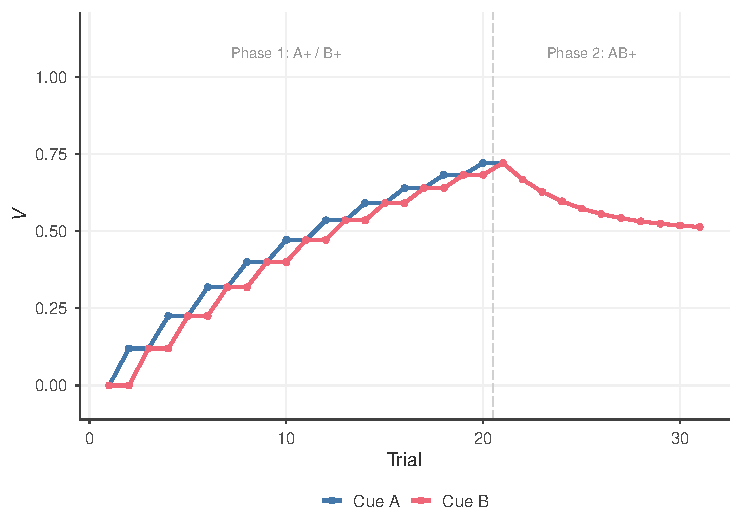
\includegraphics[width=0.7\linewidth]{Figures/fig3_overexpectation.pdf}
\caption{Overexpectation under the Rescorla-Wagner model. In Phase~1, cues A and B are each trained separately (alternating A+ and B+, 10 trials each) to $V \approx 0.72$. In Phase~2, the compound AB+ causes both $V_A$ and $V_B$ to \emph{decline} despite continued reinforcement, because $\Sigma V \approx 1.44 > \lambda = 1.0$ generates negative prediction error.}
\label{fig:overexpectation}
\end{figure}

The formalization ladder and the thinking skills demonstrated in this section are not specific to associative learning. If the reader's model is a drift-diffusion model, a Bayesian learner, or a reinforcement learning agent, the process is the same: identify the equations, specify all parameters and initial conditions, define the event structure, implement the update rule, step through the sequence, and, critically, predict the outcome before running the simulation. The specific content differs across domains, but the critical question is always whether all theoretical commitments have been made explicit in the code.

\section{Sharpening the Question: Simulation as Theory Comparison}

Section~2 equipped the reader to simulate a single model and discover its predictions. But suppose the model matches the data. Can the theory be declared correct? No; alternatives have not been excluded. A model that fits data has survived one easy exam \citep{roberts2000persuasive}. The real power of simulation lies not in confirming a model but in finding ways to distinguish it from competitors.

The contrast between Rescorla-Wagner and Mackintosh is not merely a dispute within associative learning. It embodies a tension that recurs across behavioral science: is a failure of performance caused by the \emph{absence of a signal} or by the \emph{inability to use it}? In memory research, the analogous question is whether forgetting reflects a failure of encoding or a failure of retrieval \citep{tulving1973encoding}. In decision-making, the question is whether poor choices reflect low evidence quality or a poorly placed decision criterion \citep{ratcliff2008diffusion}. In clinical psychology, the question is whether maladaptive behavior persists because the corrective experience has not occurred or because the individual's attention is not directed toward the corrective information. The simulation thinking cycle developed here is domain-general precisely because these structural tensions are domain-general. The specific models will differ; the practice of formalizing competing mechanisms, simulating them under identical conditions, and designing tests that exploit their divergences applies wherever two explanations invoke different underlying processes.

This brings the analysis to the second iteration of the Simulation Thinking Cycle. The question is now comparative: can the models be distinguished, and how? This requires implementing two models side by side, predicting whether they will agree or disagree, and reflecting on what agreement or disagreement reveals about the theories' structural commitments.

\subsection{Why One Model Is Not Enough}

Model mimicry is the norm in behavioral science \citep{jones2014unfalsifiability, pitt2002toward}. Two models built on different theoretical assumptions can produce indistinguishable predictions across standard designs. Discovering this underdetermination is itself an important finding \citep{navarro2019devil}. Simulation makes it visible. The disciplined response is not despair but precision: find the conditions under which the theories diverge, and design experiments that target those conditions.

\subsection{Adding a Competitor: Fair Comparison}

Good model comparison requires treating every model fairly, giving it its best chance, not setting up a straw man \citep{kruschke2008models}. The Mackintosh (1975) attention model \citep{mackintosh1975theory} makes a fundamentally different claim from Rescorla-Wagner. Table~\ref{tab:model_comparison} summarizes the key contrasts.

\begin{table}[t]
\centering
\small
\caption{Structural comparison of the Rescorla-Wagner and Mackintosh models. Each row represents a theoretical commitment that distinguishes the models.}
\label{tab:model_comparison}
\begin{tabular}{lll}
\toprule
\textbf{Dimension} & \textbf{Rescorla-Wagner} & \textbf{Mackintosh} \\
\midrule
Error term & Global: $\lambda - \Sigma V$ & Local: $\lambda - V_i$ \\
Learning rate ($\alpha$) & Fixed & Variable \\
What $\alpha$ tracks & Nothing & Relative predictiveness \\
V update & $\alpha_i \beta (\lambda - \Sigma V)$ & $S_i \alpha_i (\lambda - V_i)$ \\
Blocking mechanism & Error consumed & Attention withdrawn \\
\bottomrule
\end{tabular}
\end{table}

The Mackintosh model's core equations are:
\begin{align}
\Delta V_i &= S_i \cdot \alpha_i \cdot (\lambda - V_i) \label{eq:mack} \\
\alpha_i &\leftarrow
\begin{cases}
\alpha_i + \beta_{\text{up}} (1 - \alpha_i) & \text{if } |\lambda - V_i| < |\lambda - \Sigma V_{\neg i}| \\
\alpha_i - \beta_{\text{down}} \cdot \alpha_i & \text{otherwise}
\end{cases} \label{eq:mack_alpha}
\end{align}
where $\Sigma V_{\neg i}$ is the summed associative strength of all present cues except $i$, and $\beta_{\text{up}} < \beta_{\text{down}}$ reflects the theoretical assumption that attention is easier to lose than to gain \citep{lepelley2004role}.

The corresponding code makes the structural contrast with Rescorla-Wagner explicit:
\begin{verbatim}
# Mackintosh V update: LOCAL error
for (cue in cues_present) {
  V[cue] <- V[cue] + S[cue] * alpha[cue] *
                      (lambda - V[cue])
}
# Alpha update: reward good predictors
for (cue in cues_present) {
  error_i     <- abs(lambda - V_old[cue])
  error_other <- abs(lambda - sum(V_old[others]))
  if (error_i < error_other) {
    alpha[cue] <- alpha[cue] +
                   beta_up * (1 - alpha[cue])
  } else {
    alpha[cue] <- alpha[cue] -
                   beta_down * alpha[cue]
  }
}
\end{verbatim}
Comparing this with the Rescorla-Wagner code from Section~2.1 reveals the structural commitments at a glance. The V update uses $(\lambda - V_i)$ rather than $(\lambda - \Sigma V)$: local error rather than global. The alpha update loop has no counterpart in Rescorla-Wagner, where $\alpha$ is fixed. These are not incidental implementation details; they are the formal expressions of fundamentally different theoretical claims about what drives learning.

The critical structural difference is the error term: $(\lambda - V_i)$ versus $(\lambda - \Sigma V)$. On the first AB+ trial after Phase~1, when $V_A \approx 0.72$ and $V_B = 0$, the RW update for B is $0.4 \times 0.3 \times 0.278 = 0.033$, whereas the Mackintosh update is $0.3 \times 0.5 \times 1.0 = 0.15$, roughly four times larger. In RW, A's prior learning has consumed the error signal. In Mackintosh, B's local error is unaffected by A's success.

This is a pedagogical implementation of the Mackintosh model, chosen to sharpen the contrast with Rescorla-Wagner. It captures the core mechanism (attention shifts toward the best predictor) but simplifies certain details. This implementation follows the parameterization of \citet{lepelley2004role}, who formalized Mackintosh's (1975) qualitative attention rule into the specific update equations used here. The original Mackintosh model did not specify the precise functional form of attention change or the separation of $S$ and $\alpha$ parameters; these are due to Le Pelley's formalization. Domain specialists should consult \citet{lepelley2004role} and \citet{wills2020progress} for discussions of alternative parameterizations. Other attention-based models include \citet{pearce1980model} and \citet{kruschke2001toward}.

\emph{Prediction checkpoint.} Both models produce ``blocking.'' But do they agree quantitatively? The reader should predict whether $V_B$ at the end of Phase~2 will be similar or very different between the two models.

Running both models on the blocking design reveals that under RW, $V_B \approx 0.13$, while under Mackintosh, $V_B \approx 0.57$. Both produce blocking, but the internal states differ profoundly. In RW, the value is low because the error is tiny. In Mackintosh, the value is moderate because the local error is large, but $\alpha_B$ has dropped from 0.50 to approximately 0.10.

\subsection{The Commitment Anatomy of a Model}

Before designing a critical test, I introduce a framework for understanding what a simulation actually tests. Most computational models can be usefully decomposed into three layers of commitment, though the boundaries between layers are not always sharp and may shift with the research question.

The core/auxiliary decomposition is investigative, not just classificatory. Researchers rarely know in advance which assumptions are load-bearing; the decomposition emerges through the simulation work itself. Ablation, parameter sweeps, and structural substitution (Section~4) are the tools that reveal which commitments carry explanatory weight and which serve only as computational scaffolding.

This decomposition has roots in the philosophy of science. \citet{lakatos1970falsification} distinguished between the \emph{hard core} of a research programme (the central claims its proponents refuse to abandon) and the \emph{protective belt} of auxiliary hypotheses that can be modified in response to anomalies. The framework I develop here translates Lakatos's distinction into the language of computational modeling and adds a third layer (implementation choices) that Lakatos did not consider, since he was not reasoning about executable code. The translation is not merely terminological. Computational models make the core/auxiliary boundary \emph{operational}: one can systematically modify each assumption, re-simulate, and observe whether the prediction changes, a procedure that is difficult to carry out through verbal reasoning alone.

The first layer is the \emph{core theoretical claim}: the mechanism the theory asserts. For Rescorla-Wagner: ``learning is driven by prediction error.'' For Mackintosh: ``attention shifts toward the most informative predictor.''

The second layer contains \emph{auxiliary assumptions}: structural choices necessary for implementation but not entailed by the core claim. In RW, the assumption that absent cues are not updated is auxiliary; \citet{vanhamme1994cue} modified precisely this assumption while preserving the prediction error core. Similarly, \citet{wagner1981sop} proposed the SOP model, replacing the error term with a memory-based mechanism while retaining associative principles, and \citet{miller1988comparator} proposed the comparator hypothesis, changing the response rule rather than the learning rule.

The third layer contains \emph{implementation choices}: parameter values ($\alpha = 0.4$), initial conditions ($V = 0$), trial counts. These carry no theoretical weight but must be specified.

The layers matter because they determine what one learns when a simulation fails. If an auxiliary assumption fails, it can be modified while preserving the core, as Van~Hamme and Wasserman did. If the core claim fails across all auxiliary variants, the theory itself is in trouble \citep{miller1995assessment}. Simulation helps localize the failure by systematically modifying one assumption at a time.

This framework also illuminates the relationships between models. Rescorla-Wagner and Mackintosh differ in their core claims, but share auxiliary assumptions. The Pearce-Hall model \citep{pearce1980model} shares Mackintosh's commitment to variable attention but differs in what $\alpha$ tracks: Mackintosh says relative predictive success; Pearce-Hall says absolute prediction error (surprise). This three-model landscape illustrates that ``model comparison'' can mean comparing different core theories or different auxiliary implementations of the same core idea. The simulation thinker must know which comparison is being made. I chose Mackintosh rather than Pearce-Hall as the running comparator because the Rescorla-Wagner/Mackintosh contrast involves a cleaner difference in core mechanism (global versus local error, fixed versus variable attention), producing a more pedagogically transparent critical test. A Rescorla-Wagner/Pearce-Hall comparison would be equally valid but would require additional exposition of Pearce-Hall's distinctive prediction that attention \emph{increases} to surprising stimuli (the opposite of Mackintosh's rule), which, while fascinating, would lengthen the tutorial substantially.

The boundary between core and auxiliary is not always sharp, and that is part of the point. Whether the global error term is ``core'' to Rescorla-Wagner or merely an auxiliary implementation of the deeper idea of prediction-error-driven learning is a substantive theoretical question, not a notational convenience. Different theorists may draw the line differently, and that disagreement is itself informative about the state of the theory. The payoff is not a definitive classification but a forced conversation about which commitment is doing the explanatory work: when a model fails, which commitment is responsible?

The core/auxiliary boundary is not merely contestable in general; it shifts systematically with the research question. Consider the global versus local error term. For a researcher studying \emph{compound conditioning} (how cues interact during learning), the distinction between $\lambda - \Sigma V$ and $\lambda - V_i$ is core, because it determines whether cues compete for a shared teaching signal. But for a researcher studying \emph{single-cue acquisition}, the distinction is invisible: with only one cue present, global and local error are identical. The same formal assumption is core for one question and irrelevant for another.

This question-relativity has a practical implication for simulation thinking. When constructing a model, the researcher should not begin by listing all possible assumptions and choosing among them. The researcher should begin with the question and ask: which assumptions does this question \emph{require me to specify}? Which distinctions does this question make load-bearing? A model that is adequate for one question may be inappropriate for another, not because it is wrong, but because it makes the wrong things explicit and leaves the wrong things implicit. In this sense, the research question determines what the model needs to represent, determining what entities, interactions, and timescales are admitted as relevant. A good model is always good \emph{relative to a question}.

Table~\ref{tab:commitments} decomposes both models into the three commitment layers, making explicit which assumptions are shared and which are contested.

\begin{table}[t]
\centering
\small
\caption{Commitment decomposition of the Rescorla-Wagner and Mackintosh models. Shared commitments define the common ground; contested commitments define the theoretical dispute. Modifying an auxiliary assumption (as Van Hamme \& Wasserman did) produces a new model within the same theoretical family; modifying a core commitment produces a genuinely different theory. This decomposition is a first-pass heuristic for the present research question; some placements are contestable and may shift under different questions.}
\label{tab:commitments}
\begin{tabular}{p{2.5cm}p{4.5cm}p{4.5cm}}
\toprule
\textbf{Layer} & \textbf{Rescorla-Wagner} & \textbf{Mackintosh} \\
\midrule
\emph{Core claim} & Learning is driven by prediction error & Attention shifts to the best predictor \\
\midrule
\emph{Auxiliary} & Global error ($\lambda - \Sigma V$) & Local error ($\lambda - V_i$) \\
 & $\alpha$ is fixed & $\alpha$ changes with experience \\
 & Absent cues not updated & Absent cues not updated \\
 & Trial-by-trial updating & Trial-by-trial updating \\
 & Discrete cue representation & Discrete cue representation \\
\midrule
\emph{Implementation} & $\alpha_A = 0.4$, $\beta = 0.3$ & $S = 0.3$, $\beta_{\text{up}} = 0.03$ \\
 & $V_0 = 0$, 10 trials/phase & $\alpha_0 = 0.5$, $\beta_{\text{down}} = 0.15$ \\
\bottomrule
\end{tabular}
\end{table}

When simulation produces a surprising result, a diagnostic procedure applies: identify the surprise; list every commitment in the model; for each, ask whether changing it alone would eliminate the surprise; if the surprise traces to an auxiliary assumption, the core theory is not necessarily wrong; if it persists across all auxiliary variants, the core theory is in trouble. This procedure directly confronts the Duhem-Quine problem \citep{duhem1954aim}: when a model's prediction fails empirically, one can always blame an auxiliary assumption rather than the core claim. Simulation does not solve this problem (no methodology can), but it provides a structured way to investigate it. By re-simulating with modified auxiliaries, one can determine which assumptions are load-bearing and which are dispensable, narrowing the space of viable explanations far more efficiently than verbal argument alone.

\subsection{Designing a Critical Test: The Thinking Process}

This section demonstrates how simulation thinking transforms model comparison into experimental design, following five systematic steps.

\textbf{Step 1: Examine where the models agree and disagree.} Both produce blocking, but their internal states differ. In RW, $V_B \approx 0.13$ with $\alpha_B = 0.4$ (intact). In Mackintosh, $V_B \approx 0.57$ but $\alpha_B \approx 0.098$ (suppressed).

\textbf{Step 2: Interrogate the mechanisms.} In Rescorla-Wagner, blocking occurs because the global prediction error $\delta = \lambda - (V_A + V_B)$ is tiny: A's prior learning has consumed the error signal, leaving no teaching signal for any cue. B's learning rate ($\alpha_B = 0.4$) is perfectly intact; the problem is not that B cannot learn, but that there is nothing left to learn from. The model's ``diagnosis'' of B's failure is: \emph{value deficit}: B has low associative strength because the error that would have driven its learning was already absorbed by A.

In Mackintosh, the mechanism is fundamentally different. The local error term $(\lambda - V_B)$ is large throughout Phase~2; B's own prediction error is never consumed by A, because each cue has its own error term. B \emph{does} learn, reaching $V_B \approx 0.57$. But simultaneously, $\alpha_B$ declines from 0.50 to 0.098 because B is consistently a worse predictor than A (i.e., $|\lambda - V_B| > |\lambda - V_A|$ on most Phase~2 trials). The model's ``diagnosis'' of B's failure is: \emph{attention deficit}: B has reduced associative strength not because the error was absent but because the learning rate was throttled.

These are profoundly different mechanistic accounts, and they leave different internal ``signatures'' on B's state at the end of Phase~2. The question for experimental design is: what situation would force these different internal signatures to produce different observable behavior?

\textbf{Step 3: Find the condition that forces the mechanistic difference to surface.} The reasoning proceeds as follows. By Phase~2's end, the two models have left B in different states: RW gives B low $V_B$ but intact $\alpha_B$; Mackintosh gives B higher $V_B$ but suppressed $\alpha_B$. A test that probes \emph{current} associative strength would not cleanly separate the models, because both predict that B elicits a weak response (albeit for different reasons). What is needed is a test that probes the \emph{capacity for future learning}: a situation where B must learn something new, so that the learning rate becomes the decisive variable.

This reasoning leads to a specific design: Phase~3 in which B is paired with an entirely new outcome. Because the outcome is novel, $V_B$ for this new association starts at zero for both models, creating a level playing field in terms of associative strength. The difference lies entirely in the learning rate parameter. Under Rescorla-Wagner, $\alpha_B$ is intact at 0.40; B can learn the new association at its full original rate. Under Mackintosh, $\alpha_B$ has been driven down to 0.098 during Phase~2; even though the prediction error is large, the suppressed attention throttles the speed of new learning. The teaching signal is there, but the suppressed learning rate prevents B from using it effectively.

Note that resetting $V_B$ to zero for the new outcome is itself a theoretical commitment: it assumes zero generalization between the old and new outcomes. If some generalization occurred, Mackintosh's higher Phase~2 $V_B$ would give it a head start in Phase~3, potentially reducing the predicted divergence. This assumption should be stated explicitly and, ideally, subjected to sensitivity analysis.

\textbf{Step 4: Simulate the critical test.}
\begin{verbatim}
V_end     <- extract_final_V(results_p12)
alpha_end <- extract_final_alpha(results_p12)
V_end["B"] <- 0  # new outcome: reset V_B
results_p3 <- mack_simulate(design_p3,
  S=c(A=0.3, B=0.3),
  alpha_init=alpha_end, V_init=V_end)
\end{verbatim}

\emph{Prediction checkpoint.} Both models start Phase~3 at $V_B = 0$. RW has $\alpha_B = 0.40$; Mackintosh has $\alpha_B \approx 0.098$. After 10 trials, which model shows faster learning?

Figure~\ref{fig:model_comparison} reveals that under RW, $V_B$ rises to 0.72; under Mackintosh, only to 0.42. RW predicts rapid acquisition; Mackintosh predicts retarded acquisition \citep{lepelley2004role, haselgrove2010overcoming, wills2020progress}.

\textbf{Step 5: Make the mechanism visible.} Figure~\ref{fig:alpha_dynamics} plots $\alpha_B$ across all three phases, showing the decline during Phase~2 and slow recovery during Phase~3.

\paragraph{Reflect.} The five-step process followed a systematic path: simulate both models, observe mechanistic differences, identify a condition that forces the difference to surface, and simulate again to verify. This is repeatable and depends not on creativity but on understanding earned through simulation. More broadly, this iteration of the cycle has shifted the \emph{Question} from ``what does the model predict?'' to ``which theory is right?'' and the \emph{Surprise} from a mismatch with intuition to a mismatch between models. The \emph{Reflect} step now asks not just ``what did I learn about my theory?'' but ``what experiment should I run next?''

\emph{Exercise 4.} Change Phase~3 to 50 trials. Do the models converge? (Expected: yes, because $\alpha_B$ recovers. The diagnostic signal is the rate, not the final level.)

It is worth revisiting the observation function from Section~2.3 in the context of this critical test, because it illustrates how the mapping from $V$ to behavior can alter the interpretation of model predictions. Under a threshold observation function with $\theta = 0.3$, the Phase~2 predictions of the two models diverge not only quantitatively but \emph{qualitatively}. In Rescorla-Wagner, $V_B \approx 0.13$ after Phase~2, which falls below the threshold: B produces no conditioned response. In Mackintosh, $V_B \approx 0.57$, which exceeds the threshold: B \emph{does} produce a conditioned response. The same pair of models that both produce blocking (in the sense that $V_B$ is reduced relative to a control) disagree on whether B responds at all once behavior is measured through a nonlinear mapping. This means the observation function is not a downstream convenience to be specified later; it can determine which model appears to fit the data, and should therefore be considered as part of the experimental design, not as an afterthought.

Figure~\ref{fig:obs_impact} makes this visible. Under both models, Phase~2 involves AB+ compound trials after Phase~1 pre-training of A alone. In raw $V$ terms, both models produce ``blocking'': $V_B$ is lower than it would have been without A's pre-training. But the Mackintosh model's local error allows $V_B$ to reach 0.57, well above a plausible response threshold of $\theta = 0.3$, whereas the Rescorla-Wagner model's global error keeps $V_B$ at 0.13, below that threshold. The same two models, applied to the same design, produce opposite behavioral predictions (one predicts responding, the other predicts no responding) purely because of how the internal variable maps onto behavior. This is not a minor quantitative difference; it is a qualitative behavioral difference that could determine the outcome of an empirical test.

\begin{figure}[t]
\centering
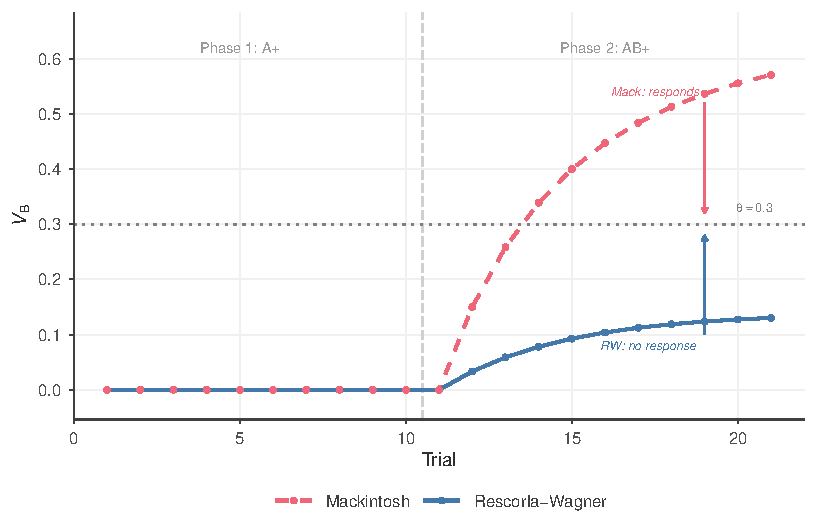
\includegraphics[width=0.75\linewidth]{Figures/fig10_obs_function_impact.pdf}
\caption{The observation function determines which model ``fits.'' Both models produce blocking in raw $V$ terms, but the Mackintosh model's $V_B$ (0.57) exceeds a response threshold ($\theta = 0.3$, dotted line), predicting a conditioned response, whereas the Rescorla-Wagner model's $V_B$ (0.13) falls below threshold, predicting no response. The same internal dynamics produce opposite behavioral predictions under a nonlinear observation function.}
\label{fig:obs_impact}
\end{figure}

This process applies wherever competing models exist. In decision-making, drift-diffusion and linear ballistic accumulator models agree on mean RTs but diverge on distributions \citep{ratcliff2008diffusion, brown2008ballistic, navarro2009fast}. In memory, exemplar and prototype models agree on accuracy but differ on generalization gradients \citep{nosofsky2011generalized}. The recipe is the same \citep{busemeyer2010cognitive, daw2011trial}.

\begin{figure}[t]
\centering
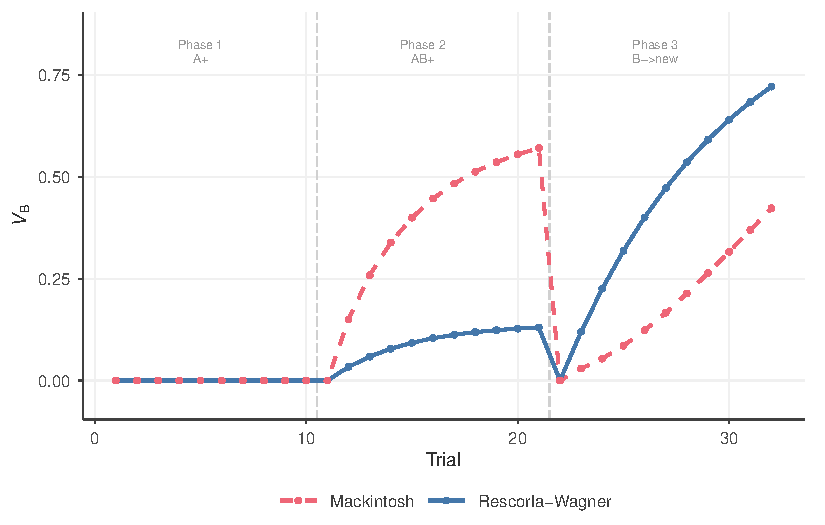
\includegraphics[width=0.85\linewidth]{Figures/fig4_critical_test.pdf}
\caption{Critical test of Rescorla-Wagner versus Mackintosh. Phase~1 trains A alone (A+); Phase~2 presents compound AB+ (blocking); Phase~3 pairs B with a new outcome (B+, with $V_B$ reset to zero). The critical divergence emerges in Phase~3: RW predicts rapid acquisition ($\alpha_B$ intact at 0.40, $V_B = 0.72$); Mackintosh predicts retarded acquisition ($\alpha_B$ suppressed to 0.098 during Phase~2, $V_B = 0.42$).}
\label{fig:model_comparison}
\end{figure}

\begin{figure}[t]
\centering
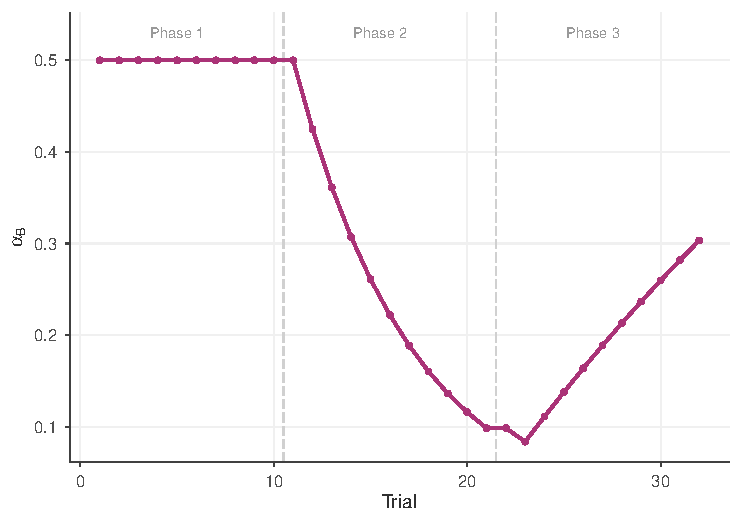
\includegraphics[width=0.65\linewidth]{Figures/fig5_alpha_dynamics.pdf}
\caption{Attention dynamics under the Mackintosh model across the three-phase blocking-plus-acquisition design. During Phase~1 (A+ only), $\alpha_B$ is stable at its initial value. During Phase~2 (AB+ compound), $\alpha_B$ declines because B is consistently a worse predictor than A. During Phase~3 (B paired with a new outcome), $\alpha_B$ begins slow recovery as B becomes the sole predictor.}
\label{fig:alpha_dynamics}
\end{figure}

\section{Stress-Testing: From Points to Spaces}

\subsection{Why Points Are Not Enough}

Until now, each simulation used specific parameter values: $\alpha_A = 0.4$, $\beta = 0.3$. But theories do not specify parameter values. The Rescorla-Wagner model asserts that learning is driven by prediction error; it does not assert that $\alpha = 0.4$. The Mackintosh model asserts that attention shifts toward the best predictor; it does not specify the rate of attention change. How much of the conclusion from Section~3 (that the blocking-plus-acquisition design dissociates the two models) comes from the theory itself, and how much is merely an artifact of arbitrary parameter choices?

This is the third iteration of the Simulation Thinking Cycle. The \emph{Question} is no longer ``what does the model predict?'' or ``where do the models diverge?'' but ``how robust is that divergence across the space of possible parameter values?'' The \emph{Formalize} step defines the parameter grid and the divergence metric. The \emph{Predict} step asks which parameters will matter most. And the \emph{Reflect} step distinguishes structural predictions from parametric coincidences.

This question is not a technicality. It is an epistemological necessity. A prediction that holds only for one specific set of parameter values is not a theoretical prediction at all; it is a parametric coincidence. To claim that a prediction follows from a theory, rather than from a particular parameterization, one must know what proportion of the parameter space supports the conclusion. Parameter sweeps are the tool that provides this warrant.

The point can be stated more sharply. When a researcher reports that ``Model A predicts X under parameters $\theta$,'' the reader has no way of knowing whether X is a consequence of the model's architecture or a consequence of $\theta$. The model's architecture (its equations, its structural assumptions) is the theoretical content. The parameters are free; they carry no theoretical commitment. A prediction that vanishes when $\alpha$ changes from 0.4 to 0.5 is not a prediction of the theory; it is a prediction of the parameterization. The only way to distinguish these cases is to explore the parameter space systematically and report the result. This is the methodological imperative that motivates the analyses in this section.

\subsection{Parameter Sensitivity Analysis}

\emph{Prediction checkpoint.} The following analysis sweeps $\alpha_A$ and $\beta$ across $[0.1, 0.9]$. The reader should predict whether the divergence will depend primarily on $\alpha_A$ or on $\beta$.

Both parameters are swept in steps of 0.05, running the full critical test at each of 289 combinations and computing $D(\theta) = |V_B^{\text{RW}} - V_B^{\text{Mack}}|$ at the end of Phase~3. The full sweep code is:
\begin{verbatim}
alpha_range <- seq(0.1, 0.9, by = 0.05)
beta_range  <- seq(0.1, 0.9, by = 0.05)
grid <- expand.grid(alpha_A = alpha_range, beta = beta_range)
grid$divergence <- NA

for (i in 1:nrow(grid)) {
  a <- grid$alpha_A[i]; b <- grid$beta[i]
  dp12 <- c(make_trials("A", 1, 20, "P1"),
            make_trials(c("A","B"), 1, 20, "P2"))
  dp3  <- make_trials("B", 1, 20, "P3")
  # RW path
  V_rw <- rw_final(dp12, alpha=c(A=a, B=0.4), beta=b)
  V_rw["B"] <- 0
  vb_rw <- rw_final(dp3, alpha=c(A=a, B=0.4),
                    beta=b, V_init=V_rw)[["B"]]
  # Mackintosh path (S yoked to beta for fair comparison)
  state <- mack_final_state(dp12, S=c(A=b, B=b),
                            alpha_init=c(A=0.5, B=0.5))
  state$V["B"] <- 0
  vb_mack <- mack_final_state(dp3, S=c(A=b, B=b),
               alpha_init=state$alpha,
               V_init=state$V)$V[["B"]]
  grid$divergence[i] <- abs(vb_rw - vb_mack)
}
\end{verbatim}
Note that in this code, the Mackintosh salience parameter $S$ is yoked to $\beta$ so that both models have comparable base learning rates. This yoking is itself a modeling choice; a different yoking scheme might produce a different landscape.

Figure~\ref{fig:heatmap} reveals the landscape. The divergence spans a broad region, confirming robustness. Notably, the divergence depends primarily on $\beta$, with $\alpha_A$ having negligible effect: $\alpha_A$ controls Phase~1 pre-training speed, and with 20 trials A reaches asymptote for most values; $\beta$ directly determines Phase~3 acquisition rate. Maximal divergence occurs at low $\beta$: when the base learning rate is small, Mackintosh's suppressed $\alpha_B$ creates a larger handicap.

\begin{figure}[t]
\centering
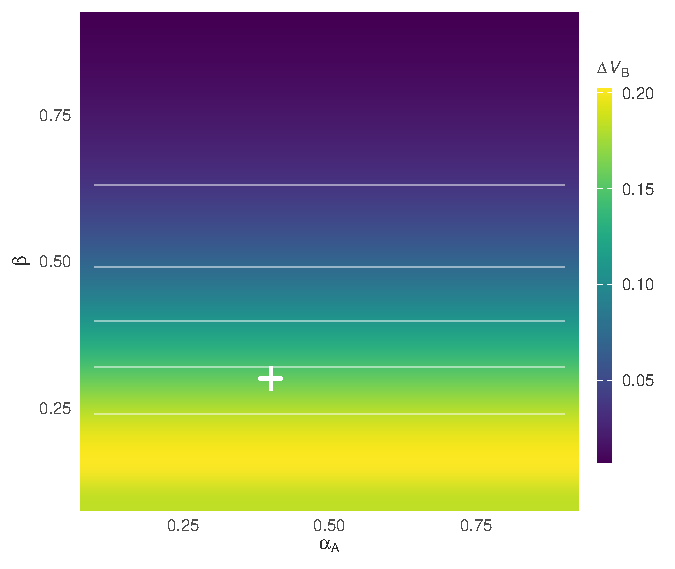
\includegraphics[width=0.65\linewidth]{Figures/fig6_param_sweep.pdf}
\caption{Parameter sensitivity analysis for the blocking-plus-acquisition critical test. Each cell shows $D(\theta) = |V_B^{\text{RW}} - V_B^{\text{Mack}}|$ at the end of Phase~3, as a function of $\alpha_A$ and $\beta$. Brighter regions indicate greater discriminability between models. The cross marks the parameters used in Section~3. Divergence depends primarily on $\beta$ (the base learning rate), with $\alpha_A$ having negligible effect once Phase~1 is long enough for A to reach asymptote.}
\label{fig:heatmap}
\end{figure}

The heatmap also reveals an unexpected asymmetry that is itself theoretically informative. The near-independence of divergence from $\alpha_A$ means that the critical test's discriminatory power is remarkably insensitive to how quickly A is pre-trained in Phase~1. Whether A learns fast ($\alpha_A = 0.9$) or slow ($\alpha_A = 0.1$), as long as Phase~1 is long enough for A to reach reasonable associative strength, the Phase~3 divergence is preserved. This robustness traces to the models' asymptotic behavior: once $V_A$ is near $\lambda$, the exact path by which it got there does not matter for the Phase~2 blocking dynamics. In contrast, $\beta$ controls the speed at which \emph{both} models learn in Phase~3, so it directly determines whether the Mackintosh model's attentional handicap produces a detectable rate difference before both models reach ceiling.

\subsection{Design Parameter Optimization}

Parameter sensitivity is only half the story. Fixing model parameters within the robust region and sweeping Phase~1 trials (5--40) and Phase~2 trials (5--40), with Phase~3 at 20, produces Figure~\ref{fig:design_sweep}. Discriminability depends primarily on Phase~2 length: more compound trials allow $\alpha_B$ to decline further. This is design analysis through simulation: before running an experiment, one can explore how design choices affect the ability to distinguish theories.

\emph{Exercise 5.} Add Phase~3 trial count as a third swept dimension. Does the optimal Phase~3 length depend on Phase~2 length?

\begin{figure}[t]
\centering
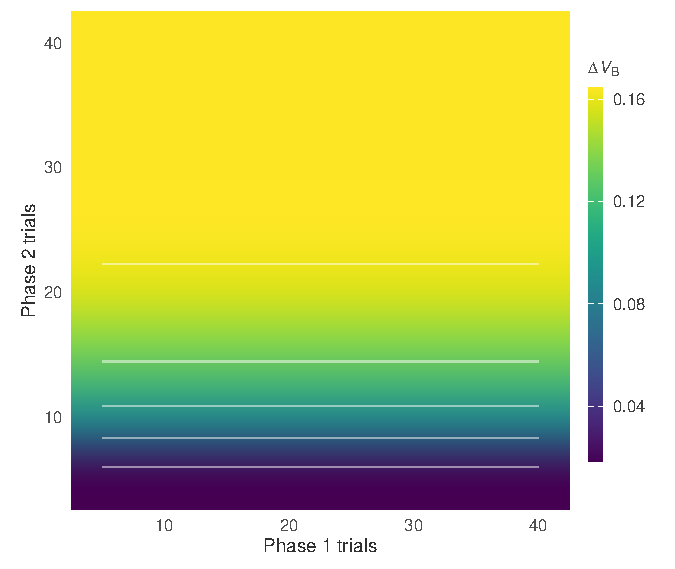
\includegraphics[width=0.65\linewidth]{Figures/fig7_design_sweep.pdf}
\caption{Design optimization for the blocking-plus-acquisition critical test. Discriminability between Rescorla-Wagner and Mackintosh ($D = |V_B^{\text{RW}} - V_B^{\text{Mack}}|$ at Phase~3 end) as a function of Phase~1 and Phase~2 trial counts, with Phase~3 fixed at 20 trials. Discriminability depends primarily on Phase~2 length: more compound trials allow the Mackintosh model's $\alpha_B$ to decline further, amplifying the Phase~3 divergence.}
\label{fig:design_sweep}
\end{figure}

The design sweep provides actionable guidance for experimental planning. A researcher who had planned a design with 10 Phase~1 trials and 5 Phase~2 trials would discover from this analysis that the experiment has low discriminatory power, not because the models do not differ in principle, but because 5 compound trials are insufficient for the Mackintosh model's attention mechanism to suppress $\alpha_B$ meaningfully. Increasing Phase~2 to 20 or more trials moves the design into the high-divergence region, substantially improving the experiment's theoretical informativeness. This is design optimization through simulation: the experimental design is itself a variable to be tuned, and simulation reveals how to tune it before any data are collected.

\subsection{When a Prediction Fails the Sweep: A Cautionary Example}

Every example so far has shown predictions that survive scrutiny: the blocking-plus-acquisition divergence holds across a broad region of parameter space. It is equally important to illustrate what happens when a prediction does \emph{not} survive, when simulation thinking reveals that a seemingly robust conclusion is actually a parametric coincidence.

Consider the overexpectation effect from Section~2.4. The verbal intuition (that two well-learned cues will lose associative strength when compounded) feels like a structural prediction, a necessary consequence of summed prediction error. But is it? A parameter sweep over $\alpha$ and $\beta$ reveals that overexpectation is pronounced only when the effective learning rate ($\alpha \beta$) is in a moderate range. When $\alpha \beta$ is very small, learning in Phase~1 is too slow for either cue to reach asymptote, so $\Sigma V$ never exceeds $\lambda$ and overexpectation does not occur. When $\alpha \beta$ is very large, both cues reach $\lambda$ quickly and then decline equally quickly in Phase~2, but the decline is so rapid that it may be undetectable in a short experiment with noisy measurements. The ``sweet spot'' for observing overexpectation (where the decline is large enough to measure but slow enough to track) occupies a moderate band of parameter space.

This is precisely the kind of discovery that simulation thinking is designed to produce. The researcher who simulates overexpectation at a single parameter set and observes a clear decline may believe the effect is robust. The researcher who sweeps the parameter space discovers that the effect is \emph{parametric}, not structural: it depends on the learning rate falling within a specific range. This does not mean overexpectation is uninteresting; it remains a genuine, empirically confirmed prediction of the model \citep{rescorla1970reduction}. But it means that reporting the prediction without reporting the parameter conditions under which it holds is incomplete. The sweep transforms the claim from ``the model predicts overexpectation'' to ``the model predicts overexpectation when $\alpha\beta \in [0.05, 0.3]$, approximately.'' The more precise claim is more useful, more honest, and more falsifiable.

Figure~\ref{fig:oe_sweep} displays the full landscape. The magnitude of the decline in $V_A$ during compound Phase~2 is plotted as a function of $\alpha$ and $\beta$. The bright (yellow) region shows parameter combinations where overexpectation is large and readily detectable. The dark (purple) region in the lower-left corner shows combinations where the effective learning rate is too low for either cue to reach asymptote in Phase~1, so the compound never overpredicts and no decline occurs. The dark region in the upper-right corner shows a subtler phenomenon: learning is so fast that the decline happens within one or two trials and may be missed entirely in a short Phase~2. The cross marks the parameters used in Section~2.4. This landscape transforms the theoretical claim: overexpectation is a genuine prediction of the Rescorla-Wagner model, but its detectability depends on where in the parameter space the researcher's participants fall. Reporting the prediction without reporting this dependence would be incomplete.

\begin{figure}[t]
\centering
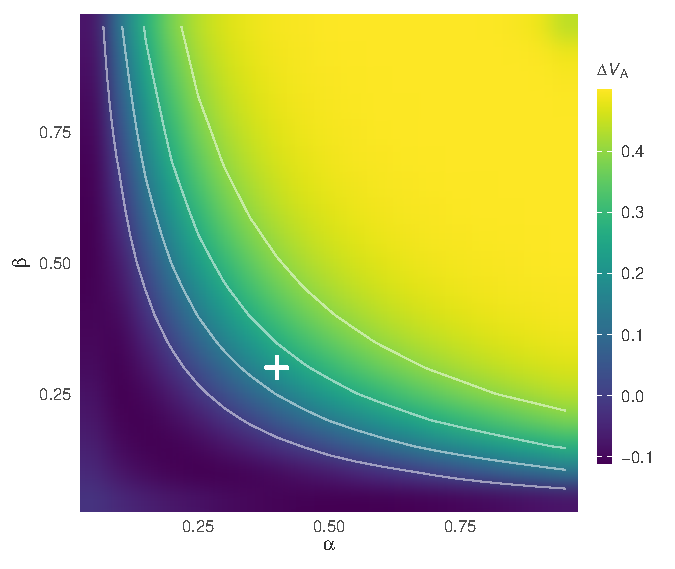
\includegraphics[width=0.65\linewidth]{Figures/fig9_overexpectation_sweep.pdf}
\caption{Overexpectation is parametric, not structural. The heatmap shows the magnitude of the decline in $V_A$ during compound AB+ trials as a function of $\alpha$ and $\beta$. Overexpectation is pronounced in the bright region (moderate to high learning rates) but vanishes in the dark lower-left corner (low learning rates, cues never reach asymptote). The cross marks the Section~2.4 parameters. This sweep reveals that overexpectation is a prediction of the model under specific parameter conditions, not an architectural inevitability.}
\label{fig:oe_sweep}
\end{figure}

\subsection{Structural Versus Parametric Predictions}

The parameter sweep performs a theoretical function, not merely a methodological one. A prediction that survives across a broad, theoretically plausible range of parameter values is a \emph{structural prediction}: it derives from the theory's architecture, from the commitments that define the model class rather than any particular instance within it. A prediction that depends on specific parameter values is a \emph{parametric prediction}: a claim about the model in one parameterization, not about the underlying theory.

This distinction maps directly onto the commitment anatomy discussed in Section~3.3. A structural prediction is a consequence of the core theoretical claim and the auxiliary assumptions; it survives variation in the implementation layer. A parametric prediction is a consequence of all three layers jointly, including the specific implementation choices. Parameter sweeps thus perform a \emph{theoretical} function: they separate the claims that follow from the theoretical commitments from the claims that follow from implementation choices. When a prediction survives the sweep, it has been promoted from ``a model result'' to ``a theoretical prediction.'' When it does not survive, the researcher has learned that what appeared to be a consequence of the theory was actually a consequence of the parameters chosen. The sweep does not merely validate the experiment; it clarifies what the theory actually says.

This distinction connects to the concept of severe testing in the philosophy of science \citep{mayo1996error}. A test is severe only if it would very probably have detected the error, were there one. A structural prediction (one that survives the full parameter space) has been tested in a spirit analogous to this: any parameter combination that could have broken the prediction has been examined and found insufficient. A parametric prediction, by contrast, has been tested only at one point, and the appearance of confirmation may be an artifact of that point's location. Parameter sweeps thus operationalize the severity criterion: they transform the philosophical intuition that ``a test should be hard to pass'' into a quantitative assessment of how much of the possibility space supports the conclusion.

The distinction is idealized: many predictions are neither fully structural nor merely pointwise, but robust over some regions and fragile over others. What counts as a theoretically plausible parameter range is itself question-relative and should be justified. Predictions that survive broad and theoretically relevant sweeps have a stronger claim to being theoretical; predictions that survive only narrow regions should be reported as conditional on those regions. In every case: think in spaces, not points.

\paragraph{Reflect.} This third iteration of the cycle has changed the nature of the conclusion. In Section~2, the conclusion was ``the model predicts X.'' In Section~3, it was ``the models diverge under condition Y.'' Now, in Section~4, the conclusion is ``the divergence is a structural property of the theories, not an artifact of the parameters I chose.'' Each pass through the cycle has raised the epistemic bar: from prediction, to comparison, to robustness.

\subsection{Isolating Mechanism Contributions Through Simulation}

The models considered in this tutorial contain multiple interacting mechanisms. In the Mackintosh model, the V update (local error drives associative change) and the $\alpha$ update (attention shifts toward the best predictor) are two distinct mechanisms that jointly produce behavior. Blocking under Mackintosh is not a consequence of either mechanism alone; it is an \emph{emergent} property of their interaction. The V update allows B to learn (local error is large), while the $\alpha$ update simultaneously throttles B's future learning rate. Neither mechanism in isolation produces the distinctive Phase~3 prediction.

Simulation provides a direct method for isolating mechanism contributions: disable one mechanism and observe how the model's behavior changes. Figure~\ref{fig:isolation} demonstrates this for the Phase~3 critical test. Three conditions are compared: the Rescorla-Wagner model (blue), the full Mackintosh model (red), and a modified Mackintosh model in which $\alpha$ is frozen at its initial value, so the attention mechanism is disabled, leaving only the local error mechanism active (green).

The result is striking. With the attention mechanism disabled, the Mackintosh model learns \emph{faster} than Rescorla-Wagner in Phase~3 ($V_B = 0.80$ versus $0.72$), because the local error term $(\lambda - V_B)$ provides a larger learning signal than the global error $(\lambda - \Sigma V)$ when $V_B$ is low. It is the attention mechanism (specifically, the suppression of $\alpha_B$ during Phase~2) that produces the retarded Phase~3 acquisition. The Phase~3 divergence between models is not a consequence of the error architecture; it is a consequence of the attention dynamics that ride on top of it.

This ablation technique (freezing one mechanism while leaving others active) generalizes to any model with multiple interacting components. In a drift-diffusion model, one can freeze the boundary while varying drift rate, or vice versa, to isolate which mechanism drives a predicted effect. In a Bayesian model, one can fix the prior and vary the likelihood, or fix the likelihood and vary the prior. The principle is the same: when a model predicts something surprising, ask which mechanism is responsible by disabling each in turn. If the prediction survives ablation of mechanism A but not mechanism B, then B is the load-bearing component. If it requires both, the prediction is genuinely emergent, a property of the interaction, not of either mechanism alone.

\begin{figure}[t]
\centering
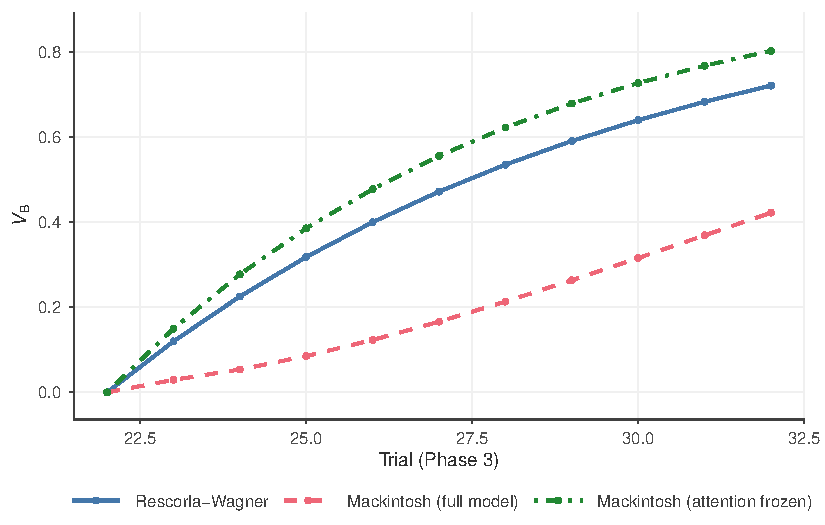
\includegraphics[width=0.75\linewidth]{Figures/fig11_mechanism_isolation.pdf}
\caption{Mechanism isolation in the Mackintosh model. Phase~3 learning of cue B under three conditions: Rescorla-Wagner (blue, $V_B = 0.72$), full Mackintosh (red, $V_B = 0.42$), and Mackintosh with the attention mechanism frozen ($\alpha_B$ held at 0.50 throughout; green, $V_B = 0.80$). With attention frozen, Mackintosh learns \emph{faster} than RW, demonstrating that the Phase~3 slowing is driven primarily by attention suppression rather than by the local error architecture.}
\label{fig:isolation}
\end{figure}

This analysis reveals something important about the commitment anatomy from Section~3.3. In the full Mackintosh model, the local error term and the attention dynamics are both listed as ``auxiliary assumptions'' in Table~\ref{tab:commitments}. But the ablation shows they play very different roles: the local error term determines the \emph{direction} of learning (positive, because $\lambda - V_B > 0$), while the attention dynamics determine the \emph{rate}. Modifying the error term would change what B learns; disabling the attention mechanism would change how fast B learns. These are not interchangeable auxiliaries; they carry different explanatory weight. The simulation-based ablation makes this weight visible in a way that inspecting the equations alone does not.

\section{Bridging to Reality: When Ideal Meets Noisy}

\subsection{From Ideal Agents to Real Participants}

Every simulation so far described an ideal agent. Real participants are noisy, heterogeneous, and bounded. Bridging this gap requires a generative model specifying three sources of variability, each a theoretical commitment: individual differences ($S_i \sim \text{Beta}(3, 7)$), model dynamics ($V_B^{(i)} = f_{\text{Mack}}(\text{design}, S_i)$), and observation noise ($Y_i = V_B^{(i)} + \epsilon_i$, $\epsilon_i \sim \mathcal{N}(0, \sigma^2)$). This is not simply noise added to the model. It is a second-order theory about how a population of agents produces observable data. \citet{yu2023fear} demonstrated that modeling individual differences in latent mechanisms was essential for disentangling processes in fear generalization.

\subsection{Simulation-Based Power Analysis}

The power of a design is the probability that a statistical test rejects the null when a specified alternative is true. Unlike formulaic power calculations \citep{cohen1992power}, simulation-based power analysis accommodates any model, design, and analysis pipeline \citep{debruine2021understanding, brysbaert2018power, green2016simr}.

\emph{Prediction checkpoint.} How many participants are needed for 80\% power: approximately 10--15, 30--50, or 100+?

For each sample size $N$ from 10 to 100, 500 experiments are simulated:
\begin{verbatim}
for (i in 1:n_subj) {
  s_i   <- rbeta(1, 3, 7)  # individual salience
  state <- mack_final_state(design_p12,
             S=c(A=s_i, B=s_i), ...)
  state$V["B"] <- 0        # new outcome
  V_end <- mack_final_state(design_p3,
             alpha_init=state$alpha,
             V_init=state$V, ...)$V
  vb_obs[i] <- V_end["B"] + rnorm(1, 0, noise_sd)
}
p <- t.test(vb_obs, mu=vb_rw_ref,
            alternative="less")$p.value
\end{verbatim}

Figure~\ref{fig:power} shows the power curve. Power crosses 80\% at approximately $N = 30$ participants, indicating practical feasibility. The curve also reveals something about the theory: strong predictions require few participants; diffuse predictions require many more.

The shape of the power curve is itself informative. The steep initial rise indicates that the effect is reasonably large; even small samples provide non-trivial power. The gradual flattening beyond 50 participants indicates diminishing returns: doubling the sample size from 50 to 100 buys only a few additional percentage points of power. When the power curve is steep, the experiment is forgiving of slight underpowering; when it is flat near the target, precise sample size determination matters less.

But the power curve also forces a confrontation with a deeper question. When power is low, two fundamentally different diagnoses are possible. The first is that the noise is too large, a measurement problem addressable by better instruments or more controlled conditions. The second is that the theoretical prediction itself is too weak: the models may be more similar than believed, the design may not probe the right variable, or the theory's claims may be inherently subtle for this type of data. These diagnoses call for different responses: better measurement versus deeper theorizing. The power curve does not tell the researcher which diagnosis applies, but it forces the question to be asked.

The Monte Carlo methodology underlying this power analysis deserves brief comment. Each power estimate is a sample proportion: the fraction of simulated experiments in which $p < 0.05$. The standard error of this estimate is $\text{SE} = \sqrt{\hat{p}(1-\hat{p})/N_{\text{sim}}}$, where $N_{\text{sim}}$ is the number of simulated experiments. With 500 simulations and an estimated power of 0.80, the standard error is $\sqrt{0.80 \times 0.20 / 500} = 0.018$, giving a 95\% confidence interval of approximately $[0.76, 0.84]$. This precision is adequate for design decisions. In practice, 500--1000 simulations provide a reliable basis for deciding whether to proceed; more are needed only when power is near a decision boundary.

The same discipline from Section~4 applies: the power analysis should be stress-tested by varying noise, individual-differences distributions, and Phase~3 length.

\emph{Exercise 6.} Increase noise from $\sigma = 1.0$ to $\sigma = 3.0$ and rerun. How many additional participants are needed?

\begin{figure}[t]
\centering
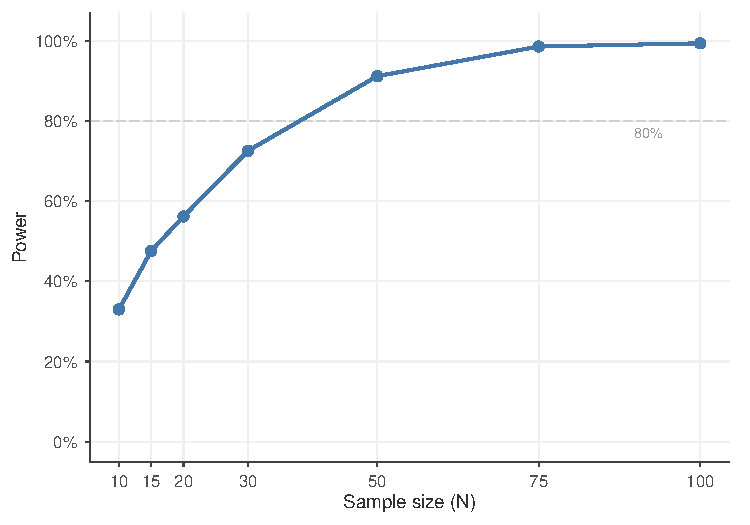
\includegraphics[width=0.65\linewidth]{Figures/fig8_power_curve.pdf}
\caption{Simulation-based power analysis for the blocking-plus-acquisition critical test. The curve shows the probability that a one-sample $t$-test detects slower Phase~3 acquisition (relative to the RW prediction) as a function of sample size, when the Mackintosh model is the true data-generating process. Individual salience varies as $S_i \sim \text{Beta}(3,7)$ with observation noise $\sigma = 1.0$. Dashed line marks 80\% power, crossed at approximately $N = 30$ participants.}
\label{fig:power}
\end{figure}

\subsection{Further Directions}

This tutorial has focused on simulation for theoretical reasoning. Three downstream applications deserve brief mention. \emph{Model and parameter recovery}: before trusting model-based conclusions, one should verify that the analysis correctly identifies the generating model and recovers its parameters \citep{wilson2019ten}. \emph{Simulation-based inference}: if one can simulate from a model, one can do inference without a likelihood function, using Approximate Bayesian Computation \citep{sunnaker2013abc, turner2012tutorial} or neural density estimation \citep{cranmer2020frontier}. \emph{Open science}: simulation code specifying a generative model, design, and analysis plan constitutes the core of a pre-registration \citep{nosek2018preregistration, schad2021workflow, munafo2017manifesto}. Each topic warrants its own tutorial; see \citet{farrell2018computational}, \citet{lee2013bayesian}, and \citet{turner2014generalized}.

The same stress-testing discipline from Section~4 applies here. The power curve shown in Figure~\ref{fig:power} rests on specific distributional assumptions: $S_i \sim \text{Beta}(3, 7)$, $\sigma = 1.0$, and 10 Phase~3 trials. Each of these is a modeling choice that could be wrong. A thorough power analysis would rerun the entire procedure under alternative assumptions: larger noise ($\sigma = 2.0$ or $3.0$), different individual-differences distributions ($\text{Beta}(2, 8)$ or $\text{Beta}(5, 5)$), and different Phase~3 lengths. A power analysis that is robust across plausible generative assumptions is a strong basis for proceeding with data collection; one that is sensitive to specific distributional choices is a warning to investigate further before committing resources.

\section*{Interlude: The Cycle Applied to a Different Model}

To illustrate that the Simulation Thinking Cycle does not depend on associative learning, I apply it to a question about the drift-diffusion model (DDM) of perceptual decision-making \citep{ratcliff2008diffusion}.

\paragraph{Question.} The DDM assumes that noisy evidence accumulates over time toward one of two decision boundaries. Raising the boundary separation $a$ is widely understood to implement a speed-accuracy tradeoff: higher $a$ means slower but more accurate decisions. But is this relationship linear? Does each unit increase in $a$ buy the same amount of accuracy?

\paragraph{Formalize.} The DDM is parameterized by drift rate $v$ (signal strength), boundary separation $a$ (caution), starting point $z$ (bias), and non-decision time $t_0$. For a simple two-choice task with $v = 1.0$, $z = a/2$ (unbiased), and $t_0 = 0.3$s, the accuracy and mean RT can be computed analytically \citep{navarro2009fast} or by simulation. The formalization step requires specifying each parameter, and noting that the starting point rule $z = a/2$ is itself an auxiliary assumption (the model could equally use an asymmetric starting point).

\paragraph{Predict.} Most researchers predict a monotonic, roughly linear speed-accuracy tradeoff: as $a$ increases from 0.5 to 3.0, both accuracy and mean RT should increase in tandem.

\paragraph{Simulate.} In pseudocode:
\begin{verbatim}
for (a in seq(0.5, 3.0, by=0.1)) {
  accuracy[a] <- ddm_accuracy(v=1, a=a, z=a/2)
  mean_rt[a]  <- ddm_mean_rt(v=1, a=a, z=a/2, t0=0.3)
}
plot(mean_rt, accuracy)
\end{verbatim}
The result reveals that the speed-accuracy tradeoff is not linear but \emph{concave}. Accuracy rises steeply at first but then asymptotes. Beyond $a \approx 2.0$, accuracy is virtually perfect, and further increases in $a$ add RT cost with negligible accuracy benefit.

For example, at $a = 0.5$, accuracy is approximately 62\% and mean RT is approximately 0.65s. At $a = 1.5$, accuracy rises to approximately 95\% and mean RT to 0.95s, a substantial improvement in accuracy for a modest cost in time. But at $a = 2.5$, accuracy is approximately 99.5\% while mean RT has risen to 1.55s. The last unit of boundary increase bought only 4.5 percentage points of accuracy at a cost of 0.6 seconds. The marginal return has collapsed.

\paragraph{Surprise and Reflect.} The diminishing-returns structure of the speed-accuracy tradeoff has practical consequences that verbal reasoning does not naturally capture. There exists an optimal regime where the tradeoff is most informative for experimental purposes: boundary values where small changes in $a$ produce measurable changes in both accuracy and RT. Outside this regime (at very low or very high $a$), one variable is at ceiling or floor, and the experiment loses sensitivity. This insight, visible only through simulation (or through the analytical formula, which most researchers do not compute), directly informs experimental design.

The same cycle (Question, Formalize, Predict, Simulate, Surprise, Reflect) structured this reasoning. The model changed entirely; the discipline did not. But it is worth noting what does change across model classes. In the associative learning examples, the Question concerned discrete cues and trial-by-trial dynamics; here it concerns a continuous accumulation process. The Formalize step required specifying a stochastic process rather than a deterministic update rule. The Surprise came from the nonlinearity of a tradeoff rather than from cue competition. And the Reflect step informed design regime selection rather than theory comparison. The cycle's six steps are invariant; the content that fills each step adapts to the model's ontology.

\section{Discussion: Principles, Pitfalls, and Practices}

The preceding sections walked through the Simulation Thinking Cycle three times (first with a single model, then with competing models, then across parameter spaces) and bridged to realistic experimental design. Table~\ref{tab:summary} summarizes the skills developed at each stage and maps them to companion code. A recurring theme across all sections has been that simulation generates \emph{epistemically productive surprise}, but the surprises differ in kind: some reveal hidden consequences of a single model (blocking, overexpectation), some expose divergences between competing mechanisms (the critical test), some uncover measurement dependence (the observation function), some distinguish structural from parametric predictions (parameter sweeps), and some reveal that a seemingly robust prediction is actually fragile (the overexpectation sweep). This section consolidates the epistemological principles that emerged from these examples, addresses practical difficulties, and discusses the scope and limits of simulation-based reasoning.

\begin{table}[t]
\centering
\small
\caption{Tutorial summary. Each section develops a specific thinking skill through a pass of the Simulation Thinking Cycle, with corresponding companion code.}
\label{tab:summary}
\begin{tabular}{p{1.2cm}p{3.2cm}p{3.5cm}p{3.5cm}}
\toprule
\textbf{Section} & \textbf{Thinking skill} & \textbf{Cycle emphasis} & \textbf{Companion code} \\
\midrule
2.1--2.2 & Formulating simulatable questions; recognizing implicit commitments & Full cycle (first pass): all six steps labeled & \texttt{analysis/01\_blocking.R} \\
2.3 & Specifying observation functions & Formalize (the model-to-data mapping) & \texttt{R/models.R}: \texttt{obs\_*} functions \\
2.4 & Discovering hidden predictions & Surprise (overexpectation) & \texttt{analysis/01\_blocking.R} \\
3.1--3.2 & Fair model comparison & Formalize (two models side by side) & \texttt{analysis/02\_critical\_test.R} \\
3.3 & Decomposing commitments (core / auxiliary / implementation) & Reflect (which layer failed?) & -- \\
3.4 & Designing critical tests & Full cycle (second pass): five-step process & \texttt{analysis/02\_critical\_test.R} \\
4 & Evaluating robustness; thinking in spaces & Full cycle (third pass): parameter sweeps & \texttt{analysis/03\_parameter\_sweep.R} \\
5 & Bridging to reality; simulation-based power & Formalize (generative model) + Simulate (Monte Carlo) & \texttt{analysis/04\_virtual\_experiment.R} \\
\bottomrule
\end{tabular}
\end{table}

\subsection{Seven Principles of Simulation Thinking}

Each principle is stated, justified, and connected to the tutorial section that demonstrates it.

\emph{Principle 1: Simulate before experimenting.} Simulation is the first step of theoretical derivation, not the last step of analysis. If a theory cannot generate predictions through simulation, it may not be precise enough to test. The blocking example (Section~2.2) illustrated that even a well-understood equation can produce predictions the theorist did not anticipate. The practical implication is direct: before committing to an experimental design, simulate the theory's predictions for that design. If the simulation reveals that the theory does not actually predict what the researcher assumed, the experiment should be redesigned before data are collected. \emph{Checklist question:} Have I written down what my model predicts for this design before running the study?

\emph{Principle 2: Simulate the competitor's theory, not just one's own.} A model that fits data has survived one easy exam \citep{roberts2000persuasive}. Scientific value comes from divergent predictions, conditions under which competing models disagree (Section~3). Fair comparison requires giving the competitor its best chance, not constructing a straw man \citep{kruschke2008models}. It is worth acknowledging that the set of competitors considered is never exhaustive; unconceived alternatives always exist. But simulating at least one serious competitor transforms the exercise from confirmation into genuine testing. \emph{Checklist question:} Have I simulated a competitor model under the same conditions, with parameters that favor it?

\emph{Principle 3: Consistency is not confirmation.} A model that reproduces a phenomenon is consistent with the data, not confirmed by it \citep{box1976science}. Multiple models may produce the same pattern; model mimicry is the norm, not the exception \citep{pitt2002toward}. When a simulation-derived prediction is subsequently confirmed empirically, the evidence is stronger if the prediction was novel (not used in constructing the model; \citep{mayo1996error}), but it is still not proof. The Duhem-Quine problem ensures that success can always be attributed to auxiliaries rather than the core claim. Parameter sweeps provide partial discipline (Section~4.4), but no amount of simulation can establish that a theory is true. Furthermore, generative success (the ability of a model to produce a phenomenon through simulation) demonstrates only that the model's mechanisms are \emph{sufficient}, not that they are \emph{necessary}. Different structures can generate the same behavior, and simulation alone cannot determine which structure is actual. \emph{Checklist question:} Could a different model produce the same prediction under the same conditions?

\emph{Principle 4: Think in spaces, not points.} A single simulation with a single set of parameters produces a point prediction. A parameter sweep produces a prediction region: the set of parameter values for which the qualitative conclusion holds. Predictions that survive broad, theoretically relevant sweeps have a stronger claim to being theoretical; predictions that survive only narrow regions should be reported as conditional (Section~4). What counts as a ``theoretically relevant'' range is itself question-relative: the plausible range for a learning rate in a fear conditioning study may differ from that in an appetitive paradigm. The practical standard is: report the region, justify its boundaries, and assess robustness within it. \emph{Checklist question:} What proportion of a theoretically plausible parameter space supports my conclusion?

\emph{Principle 5: Locate the failure.} When a model's prediction fails (whether against intuition, against data, or against a competitor), the critical question is which commitment is responsible. The three-layer decomposition (core claim, auxiliary assumptions, implementation choices; Section~3.3) provides the diagnostic framework. Modify one assumption at a time and re-simulate. If the failure traces to an auxiliary assumption, the core theory may survive. If it persists across all plausible auxiliary variants, the core theory is in trouble \citep{miller1995assessment}. This procedure directly addresses the Duhem-Quine problem: not by solving it, but by systematically narrowing the space of viable explanations \citep{duhem1954aim, lakatos1970falsification}. \emph{Checklist question:} When my model fails, can I identify which specific commitment is responsible?

\emph{Principle 6: No model meets data directly.} A model's internal variables reach observable behavior only through an observation function, and that function is itself a theoretical commitment. Different mappings can transform a quantitative difference into a qualitative one, or erase a divergence entirely (Section~2.3, Section~3.4). The observation function therefore belongs to the experimental design, not to a post-hoc analysis decision. In practice, every simulation result should be accompanied by a statement of the observation function used, and the robustness of conclusions should be assessed across at least two plausible mappings. \emph{Checklist question:} Have I stated my observation function, and does my conclusion survive an alternative mapping?

\emph{Principle 7: Simulation does not replace data.} Simulation reveals what a theory predicts; it cannot reveal whether the theory is true. A simulation that produces a surprising prediction has identified a testable hypothesis, not established a fact. The epistemic trajectory runs from simulation (deductive) to experiment (empirical) to inference (inductive), and each stage introduces new sources of uncertainty. The power analysis of Section~5 made this explicit: even a clear simulation-based divergence between models may be undetectable in noisy data with small samples. Simulation thinking is a tool for sharpening theoretical reasoning, not a substitute for empirical investigation.

\subsection{Researcher Degrees of Freedom in Simulation}

Just as statistical analyses involve choices that can inflate false-positive rates \citep{simmons2011false}, simulation-based reasoning involves analytic choices that affect conclusions. These degrees of freedom deserve explicit enumeration.

The first is \emph{competitor selection}: which alternative model is simulated alongside the preferred one? Different competitors may produce different divergence patterns, and the choice of competitor shapes the experimental design. The second is \emph{design space}: which experimental designs are explored? A researcher who sweeps only one dimension of the design space may miss the conditions under which the models agree or disagree. The third is \emph{parameter range}: the boundaries of a parameter sweep determine what counts as ``robust.'' Sweeping $\beta$ from 0.1 to 0.9 yields a different robustness assessment than sweeping from 0.01 to 0.1. The fourth is \emph{divergence metric}: the absolute difference in terminal $V_B$ used in Section~4 is one of many possible choices. A ratio, an area under the curve, or a difference in learning rate might produce a different landscape. The fifth is \emph{observation function}: as Section~3.4 demonstrated, the mapping from $V$ to behavior can qualitatively alter which model appears to fit. The sixth is \emph{sweep resolution}: a coarse grid (5 values per dimension) may miss narrow regions of divergence; a fine grid (50 values per dimension) is computationally expensive for models with many parameters.

None of these choices is inherently wrong, but each shapes the conclusions drawn. The mitigation is \emph{transparency}: report every choice, justify it where possible, and consider whether the conclusion survives alternative choices. When simulation-based reasoning is used to design an experiment or motivate a theoretical claim, the simulation code (including competitor selection, parameter ranges, divergence metric, and observation function) should be shared as part of the study's open materials. This code functions as a machine-readable pre-registration: it specifies, with a precision that no verbal protocol can match, exactly what was assumed, what was varied, and what was concluded \citep{nosek2018preregistration, schad2021workflow}. In an era when the replicability of theoretical claims matters as much as the replicability of empirical findings, transparency in simulation-based reasoning is not a luxury but a methodological obligation.

\subsection{Common Pitfalls and Practical Strategies}

\emph{``My simulation does not match my intuition; is there a bug?''} Perhaps. But before debugging the code, debug the thinking. Walk through two or three trials by hand using the model's equations (the companion function \texttt{rw\_hand\_trace()} automates this). If the hand calculations match the simulation but not the intuition, the code is correct and the intuition needs updating. This is not a failure; it is exactly the kind of theoretical insight that simulation is designed to produce.

\emph{``Both models predict the same thing.''} The condition that distinguishes them has not yet been found. The five-step critical test process from Section~3.4 provides a systematic strategy: examine the models' internal states (not just their outputs), interrogate the mechanisms that produce agreement, and find the condition that breaks the agreement. Concrete tactics include varying the number of trials per phase, varying the trial structure (add or remove phases, introduce partial reinforcement), changing the dependent variable (plot learning curves rather than endpoint values), and applying different observation functions. If after thorough exploration the models still agree, document this equivalence; it is a finding about the theoretical landscape, not a failure of the method.

\emph{``How many parameter values should I sweep?''} There is no universal answer, but two practical guidelines help. First, start with a coarse grid (e.g., 10 values per dimension) to identify the rough landscape, then refine the resolution in regions of interest. For models with more than three or four free parameters, full factorial sweeps become computationally prohibitive; in these cases, Latin hypercube sampling or adaptive grid methods can provide coverage with fewer points. Second, report the resolution and range of every sweep, so readers can assess whether the coverage was adequate.

\emph{``My model has too many free parameters.''} When a model has enough free parameters that it can produce almost any qualitative pattern, simulation thinking loses some of its diagnostic power. A parameter sweep may show that the model ``predicts'' divergent outcomes depending on which region of parameter space one examines, making it unfalsifiable in practice. In such cases, the structural versus parametric distinction (Section~4.4) becomes especially important: if a prediction survives only a small fraction of the parameter space, it is not a theoretical prediction at all \citep{pitt2002toward}. More broadly, model complexity interacts with simulation thinking in a way that mirrors its interaction with model fitting: simpler models make stronger, more falsifiable predictions, and simulation thinking is most powerful when applied to models lean enough that their predictions are genuinely constrained by their structure.

\subsection{Scope and Limitations}

This tutorial addresses simulation as a tool for theoretical reasoning: the practice of using models to think, not merely to fit. It does not cover the practical details of model fitting, Bayesian model selection, or likelihood-based comparison, which are treated thoroughly elsewhere \citep{wilson2019ten, farrell2018computational, lee2013bayesian, myung2003tutorial}. The relationship between simulation thinking and model fitting is complementary: simulation thinking determines what to expect before data are collected; model fitting determines what the data say after they arrive. Neither is sufficient without the other.

Simulation reveals \emph{what} a model predicts but not always \emph{why}. The risk that simulation becomes a computational black box (parameters in, predictions out, mechanism unexplained) is real. The Reflect step of the cycle is designed to mitigate this, but it requires active effort. The ideal practice combines simulation with analytical reasoning: simulation discovers the prediction; mathematical or logical analysis explains the mechanism \citep{navarro2021mathematical}. Simulation without understanding is computation; simulation coupled with explanation is theoretical reasoning. There is a subtler risk as well: models do not only make assumptions visible; they can also make some assumptions feel inevitable. Once a researcher has encoded agents as utility maximizers, time as discrete steps, or noise as Gaussian, these choices can sediment into seemingly natural features of the modeling landscape rather than the contestable theoretical commitments they actually are. Good simulation practice requires ongoing vigilance about which assumptions are load-bearing and which have been quietly naturalized by the model's form.

The framework developed here applies most naturally to models with well-defined equations, discrete parameters, and deterministic or parametrically stochastic dynamics. For agent-based models with emergent properties, neural network models with thousands of weights, or models exhibiting chaotic sensitivity to initial conditions, the Simulation Thinking Cycle still applies in principle (one can still question, formalize, predict, simulate, and reflect), but the parameter sweep methodology of Section~4 may require adaptation. High-dimensional parameter spaces cannot be exhaustively swept; sensitivity analysis in such cases requires more sophisticated sampling strategies or surrogate modeling approaches. These extensions are active areas of methodological research.

\subsection{Conclusion}

I have used associative learning models as the running example, but nothing in the Simulation Thinking Cycle depends on associative learning \citep{smaldino2023modeling, shiffrin2010perspectives}. The specific models were a means to an end; the thinking cycle is what should transfer. The specific equations will differ across domains; the discipline of questioning, formalizing, predicting, simulating, confronting surprise, and reflecting will not.

The broader context for this tutorial is the growing recognition that theoretical imprecision is a systemic problem in behavioral science \citep{meehl1990summaries, oberauer2019addressing, robinaugh2021invisible, eronen2021theory}. Many theories are stated with insufficient precision to generate testable predictions; many predictions are derived informally from theories that, if simulated, would predict something different. The Simulation Thinking Cycle is one response to this problem. It does not solve the theory crisis (that would require substantive theoretical work in each domain), but it provides a structured practice for ensuring that theoretical claims are as precise as the models that formalize them.

At its deepest level, the practice developed in this tutorial treats modeling not as the search for a faithful replica of reality, but as the disciplined construction of explanatory worlds: worlds in which assumptions become visible, mechanisms become testable, and structure becomes something one reasons with rather than merely codes. To think with models is to cultivate what might be called \emph{structural imagination}: the capacity to reason not in terms of variables and correlations but in terms of mechanisms, feedback, interaction, and emergence, and to ask not only ``what is actual?'' but ``what is possible, what is necessary, what is robust, and what is contingent?''

Simulation is a discipline for researchers who want their formalized theories to reveal more of their implications than verbal intuition alone can access. If the practices developed here became routine (if models were interrogated before experiments were designed, if competitor theories were simulated alongside preferred ones, and if parameter sweeps were standard before theoretical claims were published), the gap between what formalized theories entail and what researchers take them to entail would narrow substantially.

\end{linenumbers}

\section*{Declarations}

\subsection*{Funding}
K.Y. is supported by an FWO research project (G079520N) and also supported in part by the Research Fund of KU Leuven (C14/23/062).

\subsection*{Conflicts of interest}
The author declares no conflicts of interest.

\subsection*{Ethics approval}
Not applicable. This paper is a methodological tutorial involving no human participants.

\subsection*{Data availability}
All code and materials are available at \url{https://osf.io/f97rz/}.

\subsection*{Open practices statement}
All simulation code, analysis scripts, and figure-generating scripts are publicly available at \url{https://osf.io/f97rz/}. No empirical data were collected.

\subsection*{Author contributions}
K.Y. conceived the tutorial, wrote the manuscript, and developed all simulation code.

\bibliography{references}
\bibliographystyle{apalike}

\end{document}
